\documentclass[twoside]{book}

% Packages required by doxygen
\usepackage{fixltx2e}
\usepackage{calc}
\usepackage{doxygen}
\usepackage[export]{adjustbox} % also loads graphicx
\usepackage{graphicx}
\usepackage[utf8]{inputenc}
\usepackage{makeidx}
\usepackage{multicol}
\usepackage{multirow}
\PassOptionsToPackage{warn}{textcomp}
\usepackage{textcomp}
\usepackage[nointegrals]{wasysym}
\usepackage[table]{xcolor}

% Font selection
\usepackage[T1]{fontenc}
\usepackage[scaled=.90]{helvet}
\usepackage{courier}
\usepackage{amssymb}
\usepackage{sectsty}
\renewcommand{\familydefault}{\sfdefault}
\allsectionsfont{%
  \fontseries{bc}\selectfont%
  \color{darkgray}%
}
\renewcommand{\DoxyLabelFont}{%
  \fontseries{bc}\selectfont%
  \color{darkgray}%
}
\newcommand{\+}{\discretionary{\mbox{\scriptsize$\hookleftarrow$}}{}{}}

% Page & text layout
\usepackage{geometry}
\geometry{%
  a4paper,%
  top=2.5cm,%
  bottom=2.5cm,%
  left=2.5cm,%
  right=2.5cm%
}
\tolerance=750
\hfuzz=15pt
\hbadness=750
\setlength{\emergencystretch}{15pt}
\setlength{\parindent}{0cm}
\setlength{\parskip}{3ex plus 2ex minus 2ex}
\makeatletter
\renewcommand{\paragraph}{%
  \@startsection{paragraph}{4}{0ex}{-1.0ex}{1.0ex}{%
    \normalfont\normalsize\bfseries\SS@parafont%
  }%
}
\renewcommand{\subparagraph}{%
  \@startsection{subparagraph}{5}{0ex}{-1.0ex}{1.0ex}{%
    \normalfont\normalsize\bfseries\SS@subparafont%
  }%
}
\makeatother

% Headers & footers
\usepackage{fancyhdr}
\pagestyle{fancyplain}
\fancyhead[LE]{\fancyplain{}{\bfseries\thepage}}
\fancyhead[CE]{\fancyplain{}{}}
\fancyhead[RE]{\fancyplain{}{\bfseries\leftmark}}
\fancyhead[LO]{\fancyplain{}{\bfseries\rightmark}}
\fancyhead[CO]{\fancyplain{}{}}
\fancyhead[RO]{\fancyplain{}{\bfseries\thepage}}
\fancyfoot[LE]{\fancyplain{}{}}
\fancyfoot[CE]{\fancyplain{}{}}
\fancyfoot[RE]{\fancyplain{}{\bfseries\scriptsize Generated by Doxygen }}
\fancyfoot[LO]{\fancyplain{}{\bfseries\scriptsize Generated by Doxygen }}
\fancyfoot[CO]{\fancyplain{}{}}
\fancyfoot[RO]{\fancyplain{}{}}
\renewcommand{\footrulewidth}{0.4pt}
\renewcommand{\chaptermark}[1]{%
  \markboth{#1}{}%
}
\renewcommand{\sectionmark}[1]{%
  \markright{\thesection\ #1}%
}

% Indices & bibliography
\usepackage{natbib}
\usepackage[titles]{tocloft}
\setcounter{tocdepth}{3}
\setcounter{secnumdepth}{5}
\makeindex

% Hyperlinks (required, but should be loaded last)
\usepackage{ifpdf}
\ifpdf
  \usepackage[pdftex,pagebackref=true]{hyperref}
\else
  \usepackage[ps2pdf,pagebackref=true]{hyperref}
\fi
\hypersetup{%
  colorlinks=true,%
  linkcolor=blue,%
  citecolor=blue,%
  unicode%
}

% Custom commands
\newcommand{\clearemptydoublepage}{%
  \newpage{\pagestyle{empty}\cleardoublepage}%
}

\usepackage{caption}
\captionsetup{labelsep=space,justification=centering,font={bf},singlelinecheck=off,skip=4pt,position=top}

%===== C O N T E N T S =====

\begin{document}

% Titlepage & ToC
\hypersetup{pageanchor=false,
             bookmarksnumbered=true,
             pdfencoding=unicode
            }
\pagenumbering{roman}
\begin{titlepage}
\vspace*{7cm}
\begin{center}%
{\Large My Project }\\
\vspace*{1cm}
{\large Generated by Doxygen 1.8.11}\\
\end{center}
\end{titlepage}
\clearemptydoublepage
\tableofcontents
\clearemptydoublepage
\pagenumbering{arabic}
\hypersetup{pageanchor=true}

%--- Begin generated contents ---
\chapter{Compile-\/time configuration}
\label{configuration}
\hypertarget{configuration}{}
The R\+T\+OS can be configured by changing some \#define\textquotesingle{}s in p\+R\+T\+O\+S.\+h

\begin{DoxyParagraph}{global\+\_\+logging}

\end{DoxyParagraph}
All R\+T\+OS debug logging can be switched off by defining {\bfseries global\+\_\+logging} as 0 It is advised to make all application debug logging likewise dependent on this macro. Check p\+R\+T\+O\+S.\+cpp for examples

\begin{DoxyParagraph}{R\+T\+O\+S\+\_\+\+S\+T\+A\+T\+I\+S\+T\+I\+C\+S\+\_\+\+E\+N\+A\+B\+L\+ED}

\end{DoxyParagraph}
By default {\bfseries R\+T\+O\+S\+\_\+\+S\+T\+A\+T\+I\+S\+T\+I\+C\+S\+\_\+\+E\+N\+A\+B\+L\+ED} is defined as 1, which enables printing statistics for all objects. It can be defined as 0 to reduce code and data size. N\+O\+TE\+: doing so will also disable deadlock detection!

When statistics is enabled, hitting Ctrl-\/C terminates the R\+T\+OS schedular and shows the statistics.

\begin{DoxyParagraph}{R\+T\+O\+S\+\_\+\+D\+E\+F\+A\+U\+L\+T\+\_\+\+S\+T\+A\+C\+K\+\_\+\+S\+I\+ZE}

\end{DoxyParagraph}
The default stack size is 4K. You can choose another value by changing the initialization of {\bfseries R\+T\+O\+S\+\_\+\+D\+E\+F\+A\+U\+L\+T\+\_\+\+S\+T\+A\+C\+K\+\_\+\+S\+I\+ZE}.

\begin{DoxyParagraph}{R\+T\+O\+S\+\_\+\+M\+I\+N\+\_\+\+P\+R\+I\+O\+R\+I\+TY}

\end{DoxyParagraph}
The priority you can assign to a task ranges from 0 to 1000, 0 being the highest priority and 1000 the lowest. Tasks should all have a different priority. 
\chapter{Debug logging support}
\label{debug}
\hypertarget{debug}{}
The R\+T\+OS uses hwib\+::cout output stream for logging support.

The R\+T\+OS defines the trace macro, which can be used like cout, but prefixes each output with the current source file name and the current source line number. Hence (after the appropriate preparations) the statement


\begin{DoxyCode}
trace << \textcolor{stringliteral}{"n="} << n << \textcolor{stringliteral}{"\(\backslash\)n"};
\end{DoxyCode}


can create the output line


\begin{DoxyCode}
main.c:20 n=15
\end{DoxyCode}


This provides an easy way to check if and when a certain line of code is executed, and optionally print some debugging information.

Note that using the logging mechanism influences the execition of the task, maybe resulting in missing their deadlines. The suggested initialization does not implement buffering, so using cout or trace can change the timing of a task that does printing considerably.

All objects (R\+T\+OS, task, event, all waitables, mutex, pool, mailbox, channel) can be printed to an ostream using the $<$$<$ operator. Printing the R\+T\+OS will print all R\+T\+OS objects. 
\chapter{Non-\/preemptive task switching}
\label{non-preemptive}
\hypertarget{non-preemptive}{}
The R\+T\+OS uses non-\/preemptive task switching. This means that the C\+PU can be switched to another task only when the currenly executing task (directly or indirectly) calls an R\+T\+OS function. Three groups of R\+T\+OS function calls can cause such a task switch\+:


\begin{DoxyEnumerate}
\item functions that cause the current task to become non-\/runnable, like task\+::wait(), and task\+::suspend()
\item functions that make a higher-\/priority task runnable, like flag\+::set(), and task\+::resume()
\item the function task\+::release(), which only purpose is to give up the C\+PU to a higher priority task.
\end{DoxyEnumerate}

A task can be made runnable either by an excplicit action from another task, like an event\+\_\+flag\+::set() or task\+::resume() call, or implicitly by the expiration of a timer. But even for the latter case (timer expiration) the switching to another task can occur only when an R\+T\+OS function is called.

The diagram below shows the state-\/event diagram for a task. The transitions from ready to running and back are governed by the R\+T\+OS always selecting the highest-\/priority runnable task. The events that cause the transitions between runnable and blocked and vice versa, and between blocked-\/and-\/suspended and suspended are the same, they are shown in the enlarged box. A task can only get blocked by doing something (wait, read a mailbox, etc), hence there is no transition from suspended to blocked-\/and-\/suspended. 
\chapter{Latency}
\label{latency}
\hypertarget{latency}{}
When a task is activated by a timeout (either by a timer or clock, or because it is a periodic task) at a certain moment in time it will in general not be run at that time exactly, but at some later time. This delay is called the latency. Two things contribute to the latency\+:


\begin{DoxyEnumerate}
\item Higher priority taks will be run first, until no higher priority tasks are runnable.
\item When a lower priority task is running when the timer fires the R\+T\+OS will notice this only when one of the R\+T\+OS functions is called that does a rescheduling\+: task\+::wait(), flag\+::set(), task\+::suspend(), task\+::resume(), task\+::release().
\end{DoxyEnumerate}

The first contribution is a consequence of the design of the application. When you feel that it is inappropriate that a particular higher-\/priority task is run first and hence contributes to the latency of the task that is activated by the timer, you have set the task priorities wrong.

The second contribution is specific for a non-\/preemptive R\+T\+OS. (A preemptive R\+T\+OS would immediately stop (preempt) the running lower-\/priority task and switch to the higher-\/priority task.) When you have lower priority tasks in your system that use a lot of C\+PU time between the R\+T\+OS calls that do rescheduling you can insert task\+::release() calls. This call checks whether any timers that have timed out made a higher-\/priority task runnable, and if so, switches to that task.

When a task is made runnable by an explicit action of another task, for instance a task\+:resume() call or a flag\+::set() call, only the first source of delay (higher priority tasks that are runnable) is applicable, because inside such calls the R\+T\+OS will immediatley switch to the highest priority runnable task. 
\chapter{Units}
\label{units}
\hypertarget{units}{}
These constants make it easier to specify (interval) times


\begin{DoxyCode}
\textcolor{keyword}{const} \textcolor{keywordtype}{long} \textcolor{keywordtype}{long} \textcolor{keywordtype}{int}  s = ( 1000 * 1000 );
\textcolor{keyword}{const} \textcolor{keywordtype}{long} \textcolor{keywordtype}{long} \textcolor{keywordtype}{int} ms = 1000;
\textcolor{keyword}{const} \textcolor{keywordtype}{long} \textcolor{keywordtype}{long} \textcolor{keywordtype}{int} us = 1;
\end{DoxyCode}


Time in the rtos is expressed in som emultiple of microseconds, but use these constants to avoid knowledge of this detail. 
\chapter{Hierarchical Index}
\section{Class Hierarchy}
This inheritance list is sorted roughly, but not completely, alphabetically\+:\begin{DoxyCompactList}
\item \contentsline{section}{coroutine$<$ N $>$}{\pageref{classcoroutine}}{}
\item \contentsline{section}{coroutine$<$ 0 $>$}{\pageref{classcoroutine_3_010_01_4}}{}
\item \contentsline{section}{coroutine\+\_\+context}{\pageref{classcoroutine__context}}{}
\item \contentsline{section}{rtos\+:\+:event}{\pageref{classrtos_1_1event}}{}
\begin{DoxyCompactList}
\item \contentsline{section}{rtos\+:\+:waitable}{\pageref{classrtos_1_1waitable}}{}
\begin{DoxyCompactList}
\item \contentsline{section}{rtos\+:\+:channel\+\_\+base}{\pageref{classrtos_1_1channel__base}}{}
\begin{DoxyCompactList}
\item \contentsline{section}{rtos\+:\+:channel$<$ T, S\+I\+ZE $>$}{\pageref{classrtos_1_1channel}}{}
\end{DoxyCompactList}
\item \contentsline{section}{rtos\+:\+:clock}{\pageref{classrtos_1_1clock}}{}
\item \contentsline{section}{rtos\+:\+:flag}{\pageref{classrtos_1_1flag}}{}
\item \contentsline{section}{rtos\+:\+:timer}{\pageref{classrtos_1_1timer}}{}
\end{DoxyCompactList}
\end{DoxyCompactList}
\item \contentsline{section}{rtos\+:\+:mailbox\+\_\+base}{\pageref{classrtos_1_1mailbox__base}}{}
\begin{DoxyCompactList}
\item \contentsline{section}{rtos\+:\+:mailbox$<$ T $>$}{\pageref{classrtos_1_1mailbox}}{}
\end{DoxyCompactList}
\item \contentsline{section}{rtos\+:\+:mutex}{\pageref{classrtos_1_1mutex}}{}
\item \contentsline{section}{rtos\+:\+:pool\+\_\+base}{\pageref{classrtos_1_1pool__base}}{}
\begin{DoxyCompactList}
\item \contentsline{section}{rtos\+:\+:pool$<$ T $>$}{\pageref{classrtos_1_1pool}}{}
\end{DoxyCompactList}
\item \contentsline{section}{rtos}{\pageref{classrtos}}{}
\item \contentsline{section}{rtos\+:\+:task\+\_\+base}{\pageref{classrtos_1_1task__base}}{}
\begin{DoxyCompactList}
\item \contentsline{section}{rtos\+:\+:task$<$ N $>$}{\pageref{classrtos_1_1task}}{}
\end{DoxyCompactList}
\end{DoxyCompactList}

\chapter{Class Index}
\section{Class List}
Here are the classes, structs, unions and interfaces with brief descriptions\+:\begin{DoxyCompactList}
\item\contentsline{section}{\hyperlink{classrtos_1_1channel}{rtos\+::channel$<$ T, S\+I\+Z\+E $>$} \\*Waitable data queue }{\pageref{classrtos_1_1channel}}{}
\item\contentsline{section}{\hyperlink{classrtos_1_1channel__base}{rtos\+::channel\+\_\+base} \\*Rtos private implementation class }{\pageref{classrtos_1_1channel__base}}{}
\item\contentsline{section}{\hyperlink{classrtos_1_1clock}{rtos\+::clock} \\*Free-\/running clock, ticks at a fixed frequency }{\pageref{classrtos_1_1clock}}{}
\item\contentsline{section}{\hyperlink{classcoroutine}{coroutine$<$ N $>$} }{\pageref{classcoroutine}}{}
\item\contentsline{section}{\hyperlink{classcoroutine_3_010_01_4}{coroutine$<$ 0 $>$} \\*Coroutine class }{\pageref{classcoroutine_3_010_01_4}}{}
\item\contentsline{section}{\hyperlink{classcoroutine__context}{coroutine\+\_\+context} }{\pageref{classcoroutine__context}}{}
\item\contentsline{section}{\hyperlink{classrtos_1_1event}{rtos\+::event} \\*Set of things that can happen, or a thing that has happened }{\pageref{classrtos_1_1event}}{}
\item\contentsline{section}{\hyperlink{classrtos_1_1flag}{rtos\+::flag} \\*Basic synchronisation mechanism }{\pageref{classrtos_1_1flag}}{}
\item\contentsline{section}{\hyperlink{classrtos_1_1mailbox}{rtos\+::mailbox$<$ T $>$} \\*Synchronously handing over of a data item }{\pageref{classrtos_1_1mailbox}}{}
\item\contentsline{section}{\hyperlink{classrtos_1_1mailbox__base}{rtos\+::mailbox\+\_\+base} \\*Rtos private implementation class }{\pageref{classrtos_1_1mailbox__base}}{}
\item\contentsline{section}{\hyperlink{classrtos_1_1mutex}{rtos\+::mutex} \\*Mutual execlusion semaphore }{\pageref{classrtos_1_1mutex}}{}
\item\contentsline{section}{\hyperlink{classrtos_1_1pool}{rtos\+::pool$<$ T $>$} \\*Place to store and rectrieve data, no built-\/in synchronisation }{\pageref{classrtos_1_1pool}}{}
\item\contentsline{section}{\hyperlink{classrtos_1_1pool__base}{rtos\+::pool\+\_\+base} \\*Rtos private implementation class }{\pageref{classrtos_1_1pool__base}}{}
\item\contentsline{section}{\hyperlink{classrtos}{rtos} \\*Static class, namespace-\/like container for R\+T\+OS declarations }{\pageref{classrtos}}{}
\item\contentsline{section}{\hyperlink{classrtos_1_1task}{rtos\+::task$<$ N $>$} }{\pageref{classrtos_1_1task}}{}
\item\contentsline{section}{\hyperlink{classrtos_1_1task__base}{rtos\+::task\+\_\+base} \\*Independent thread of execution }{\pageref{classrtos_1_1task__base}}{}
\item\contentsline{section}{\hyperlink{classrtos_1_1timer}{rtos\+::timer} \\*One-\/short timer }{\pageref{classrtos_1_1timer}}{}
\item\contentsline{section}{\hyperlink{classrtos_1_1waitable}{rtos\+::waitable} \\*Abstract thing that a task can wait for }{\pageref{classrtos_1_1waitable}}{}
\end{DoxyCompactList}

\chapter{Class Documentation}
\hypertarget{classrtos_1_1channel}{}\section{rtos\+:\+:channel$<$ T, S\+I\+ZE $>$ Class Template Reference}
\label{classrtos_1_1channel}\index{rtos\+::channel$<$ T, S\+I\+Z\+E $>$@{rtos\+::channel$<$ T, S\+I\+Z\+E $>$}}


waitable data queue  




{\ttfamily \#include $<$rtos.\+hpp$>$}

Inheritance diagram for rtos\+:\+:channel$<$ T, S\+I\+ZE $>$\+:\begin{figure}[H]
\begin{center}
\leavevmode
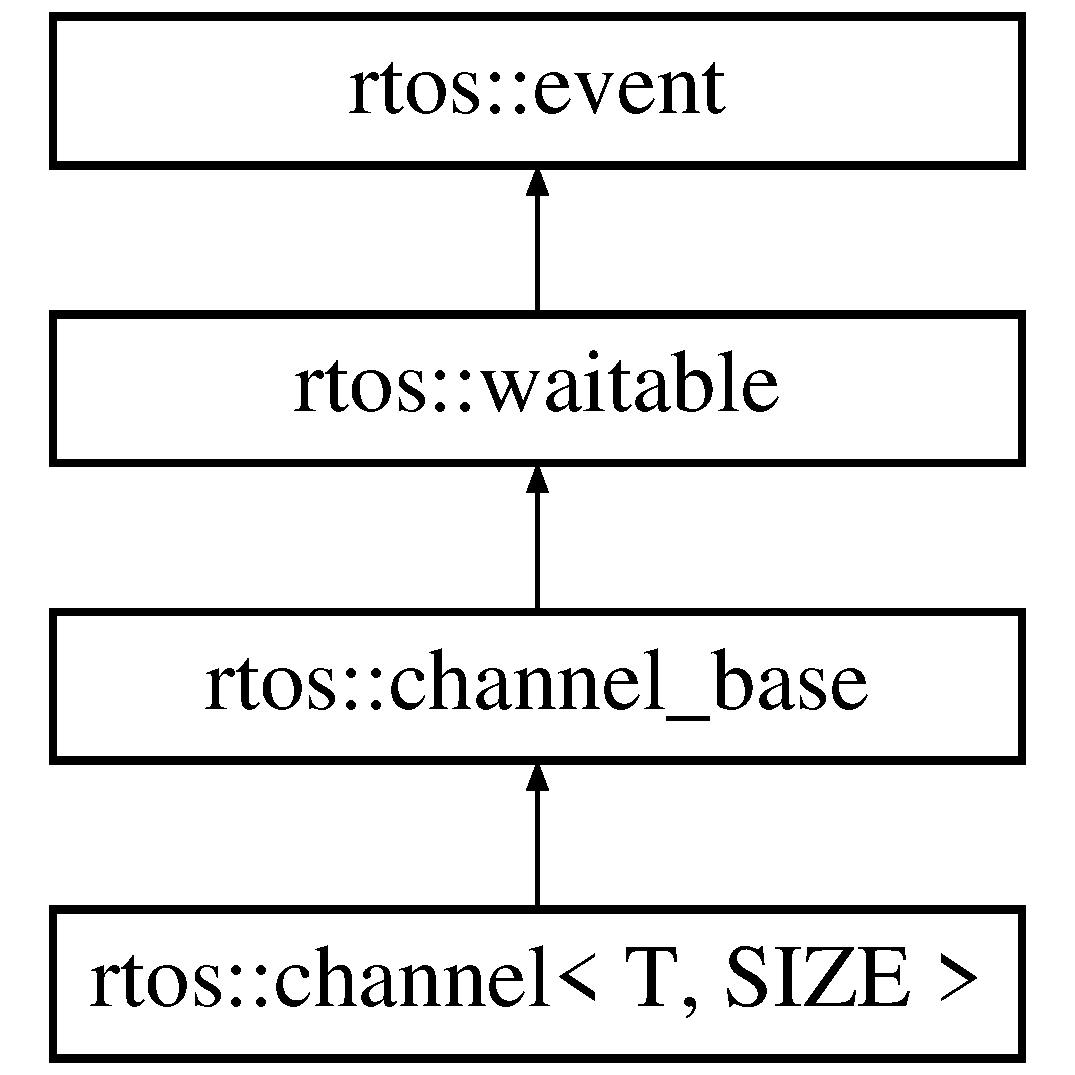
\includegraphics[height=4.000000cm]{classrtos_1_1channel}
\end{center}
\end{figure}
\subsection*{Public Member Functions}
\begin{DoxyCompactItemize}
\item 
\hyperlink{classrtos_1_1channel_a87ceb9b710e5f20399ff35be85b21bd4}{channel} (\hyperlink{classrtos_1_1task__base}{task\+\_\+base} $\ast$\hyperlink{classrtos_1_1event_aa83745aabc941145f00386fd63f6b557}{t}, const char $\ast$name=\char`\"{}\char`\"{})
\begin{DoxyCompactList}\small\item\em constructor, specify stored type, number of entries, and name \end{DoxyCompactList}\item 
void \hyperlink{classrtos_1_1channel_ad188535be39b5884f69e3eb8edf070d4}{write} (T item)\hypertarget{classrtos_1_1channel_ad188535be39b5884f69e3eb8edf070d4}{}\label{classrtos_1_1channel_ad188535be39b5884f69e3eb8edf070d4}

\begin{DoxyCompactList}\small\item\em write an item to the queue \end{DoxyCompactList}\item 
T \hyperlink{classrtos_1_1channel_abc5c7c3294e06bb60034ea4073f00cfc}{read} (void)\hypertarget{classrtos_1_1channel_abc5c7c3294e06bb60034ea4073f00cfc}{}\label{classrtos_1_1channel_abc5c7c3294e06bb60034ea4073f00cfc}

\begin{DoxyCompactList}\small\item\em read an item from the queue \end{DoxyCompactList}\item 
void \hyperlink{classrtos_1_1channel_a0a86102d13f98ef7258a3fadbc881abd}{clear} (void)
\begin{DoxyCompactList}\small\item\em clear the waitable \end{DoxyCompactList}\end{DoxyCompactItemize}
\subsection*{Additional Inherited Members}


\subsection{Detailed Description}
\subsubsection*{template$<$class T, const int S\+I\+ZE$>$\\*
class rtos\+::channel$<$ T, S\+I\+Z\+E $>$}

waitable data queue 

The (communication) channel is a template class that stores a queue of values. Values can be written at the tail of the queue, up to the number of entries for which the channel was created. It is an error to write to a channel that is full. Writes are not blocking. Any task can write to a channel.

A channel is created for a particular task. Only this owner task can read from the channel. A read will block until an entry is available. Reads are from the head of the queue.

A channel is a waitable, so the task that owns the channel can wait for the channel to be non-\/empty, after which a read from a channel will be non-\/blocking (because the channel is not empty). After a wait() that returns the channel\textquotesingle{}s event, the channel will set itself again (because the wait did not cause it to become empty). Only a read that results in an empty queue will clear the channel.

The example below shows how writing to cout can be buffered by first writing to a 2kB channel, and reading from that channel at a maximum of one character per 2 MS. The U\+A\+RT hardware in the L\+P\+C2148 chip buffers one character, which at default baudrate (38k4) takes $\sim$ 1 MS to write. So by writing at a maximum rate of one character per 2 MS no blocking will occur.


\begin{DoxyCode}
\textcolor{keyword}{class }output\_class : \textcolor{keyword}{public} task \{
\textcolor{keyword}{public}:
   channel< char, 2048 > buffer( \textcolor{keyword}{this}, \textcolor{stringliteral}{"buffer"} );
   timer hartbeat( \textcolor{keyword}{this}, \textcolor{stringliteral}{"hartbeat"} );
   \textcolor{keywordtype}{void} main( \textcolor{keywordtype}{void} )\{
      \textcolor{keywordflow}{for}( ; ; ) \{
         wait( buffer );
         cout << buffer.get();
         timer.set( 2 MS );
         wait( timer );
     \}
   \}
\}

output\_class output;

\textcolor{keywordtype}{void} print( \textcolor{keywordtype}{char} * s )\{
   \textcolor{keywordflow}{while}( *s != \textcolor{charliteral}{'\(\backslash\)0'} ) \{ output.buffer.write( *s++ ); \}
\}
\end{DoxyCode}
 

\subsection{Constructor \& Destructor Documentation}
\index{rtos\+::channel@{rtos\+::channel}!channel@{channel}}
\index{channel@{channel}!rtos\+::channel@{rtos\+::channel}}
\subsubsection[{\texorpdfstring{channel(task\+\_\+base $\ast$t, const char $\ast$name="""")}{channel(task_base *t, const char *name="")}}]{\setlength{\rightskip}{0pt plus 5cm}template$<$class T , const int S\+I\+ZE$>$ {\bf rtos\+::channel}$<$ T, S\+I\+ZE $>$\+::{\bf channel} (
\begin{DoxyParamCaption}
\item[{{\bf task\+\_\+base} $\ast$}]{t, }
\item[{const char $\ast$}]{name = {\ttfamily \char`\"{}\char`\"{}}}
\end{DoxyParamCaption}
)\hspace{0.3cm}{\ttfamily [inline]}}\hypertarget{classrtos_1_1channel_a87ceb9b710e5f20399ff35be85b21bd4}{}\label{classrtos_1_1channel_a87ceb9b710e5f20399ff35be85b21bd4}


constructor, specify stored type, number of entries, and name 

The template argument T must be a class that has a non-\/arguments constructor and supports assignment. 

\subsection{Member Function Documentation}
\index{rtos\+::channel@{rtos\+::channel}!clear@{clear}}
\index{clear@{clear}!rtos\+::channel@{rtos\+::channel}}
\subsubsection[{\texorpdfstring{clear(void)}{clear(void)}}]{\setlength{\rightskip}{0pt plus 5cm}template$<$class T , const int S\+I\+ZE$>$ void {\bf rtos\+::channel}$<$ T, S\+I\+ZE $>$\+::clear (
\begin{DoxyParamCaption}
\item[{void}]{}
\end{DoxyParamCaption}
)\hspace{0.3cm}{\ttfamily [inline]}, {\ttfamily [virtual]}}\hypertarget{classrtos_1_1channel_a0a86102d13f98ef7258a3fadbc881abd}{}\label{classrtos_1_1channel_a0a86102d13f98ef7258a3fadbc881abd}


clear the waitable 

This is automatically doen when the waitable causes a \hyperlink{classrtos_1_1task__base_a2590ba76480cecaff66282516fbeb1bb}{task\+::wait()} call to return it. 

Reimplemented from \hyperlink{classrtos_1_1waitable_ac4630398f50ba7e661a64bfc491ffa10}{rtos\+::waitable}.



The documentation for this class was generated from the following file\+:\begin{DoxyCompactItemize}
\item 
rtos.\+hpp\end{DoxyCompactItemize}

\hypertarget{classrtos_1_1channel__base}{}\section{rtos\+:\+:channel\+\_\+base Class Reference}
\label{classrtos_1_1channel__base}\index{rtos\+::channel\+\_\+base@{rtos\+::channel\+\_\+base}}


rtos private implementation class  




{\ttfamily \#include $<$rtos.\+hpp$>$}

Inheritance diagram for rtos\+:\+:channel\+\_\+base\+:\begin{figure}[H]
\begin{center}
\leavevmode
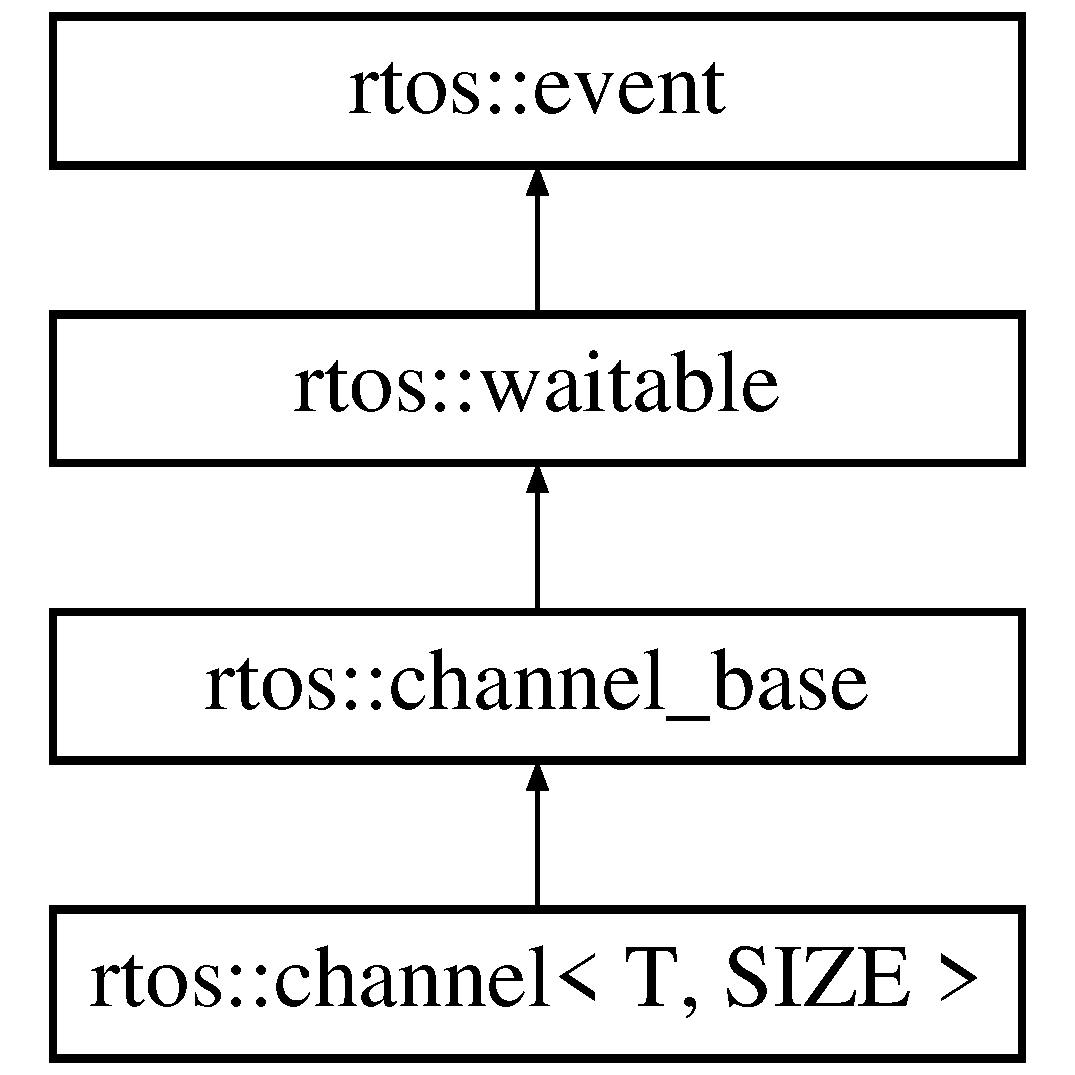
\includegraphics[height=4.000000cm]{classrtos_1_1channel__base}
\end{center}
\end{figure}
\subsection*{Public Member Functions}
\begin{DoxyCompactItemize}
\item 
void {\bfseries print} (hwlib\+::ostream \&s, bool header=true) const \hypertarget{classrtos_1_1channel__base_a2937877b07fe65fe2d3d6d69faddd9a4}{}\label{classrtos_1_1channel__base_a2937877b07fe65fe2d3d6d69faddd9a4}

\end{DoxyCompactItemize}
\subsection*{Protected Member Functions}
\begin{DoxyCompactItemize}
\item 
{\bfseries channel\+\_\+base} (\hyperlink{classrtos_1_1task__base}{task\+\_\+base} $\ast$\hyperlink{classrtos_1_1event_aa83745aabc941145f00386fd63f6b557}{t}, const char $\ast$name)\hypertarget{classrtos_1_1channel__base_a9dc28836c33737a1c14d3cac0263d07c}{}\label{classrtos_1_1channel__base_a9dc28836c33737a1c14d3cac0263d07c}

\end{DoxyCompactItemize}
\subsection*{Protected Attributes}
\begin{DoxyCompactItemize}
\item 
const char $\ast$ {\bfseries channel\+\_\+name}\hypertarget{classrtos_1_1channel__base_a3bf6e1331394d5ab745a3a7ed379350c}{}\label{classrtos_1_1channel__base_a3bf6e1331394d5ab745a3a7ed379350c}

\item 
\hyperlink{classrtos_1_1channel__base}{channel\+\_\+base} $\ast$ {\bfseries next\+\_\+channel}\hypertarget{classrtos_1_1channel__base_a5fa1e6fec7ef127baa8d5e4582c96eb6}{}\label{classrtos_1_1channel__base_a5fa1e6fec7ef127baa8d5e4582c96eb6}

\item 
int {\bfseries writes}\hypertarget{classrtos_1_1channel__base_acf4e395fcddb620239e68aacc53711d7}{}\label{classrtos_1_1channel__base_acf4e395fcddb620239e68aacc53711d7}

\item 
int {\bfseries ignores}\hypertarget{classrtos_1_1channel__base_a0dd92b2936e1e9b33990a59705e8b24f}{}\label{classrtos_1_1channel__base_a0dd92b2936e1e9b33990a59705e8b24f}

\item 
int {\bfseries q\+Size}\hypertarget{classrtos_1_1channel__base_ac7974548c1d1d39b09604640810d22cd}{}\label{classrtos_1_1channel__base_ac7974548c1d1d39b09604640810d22cd}

\item 
int {\bfseries head}\hypertarget{classrtos_1_1channel__base_a9a1e9fd7c97df262cdce5c2fc084148d}{}\label{classrtos_1_1channel__base_a9a1e9fd7c97df262cdce5c2fc084148d}

\item 
int {\bfseries tail}\hypertarget{classrtos_1_1channel__base_a220c246220377d32026f5d26c352b3dd}{}\label{classrtos_1_1channel__base_a220c246220377d32026f5d26c352b3dd}

\end{DoxyCompactItemize}
\subsection*{Friends}
\begin{DoxyCompactItemize}
\item 
class {\bfseries rtos}\hypertarget{classrtos_1_1channel__base_a2a7bcfc34141352757ad672e3ecd099f}{}\label{classrtos_1_1channel__base_a2a7bcfc34141352757ad672e3ecd099f}

\end{DoxyCompactItemize}


\subsection{Detailed Description}
rtos private implementation class 

The documentation for this class was generated from the following files\+:\begin{DoxyCompactItemize}
\item 
rtos.\+hpp\item 
rtos.\+cpp\end{DoxyCompactItemize}

\hypertarget{classrtos_1_1clock}{}\section{rtos\+:\+:clock Class Reference}
\label{classrtos_1_1clock}\index{rtos\+::clock@{rtos\+::clock}}


free-\/running clock, ticks at a fixed frequency  




{\ttfamily \#include $<$rtos.\+hpp$>$}

Inheritance diagram for rtos\+:\+:clock\+:\begin{figure}[H]
\begin{center}
\leavevmode
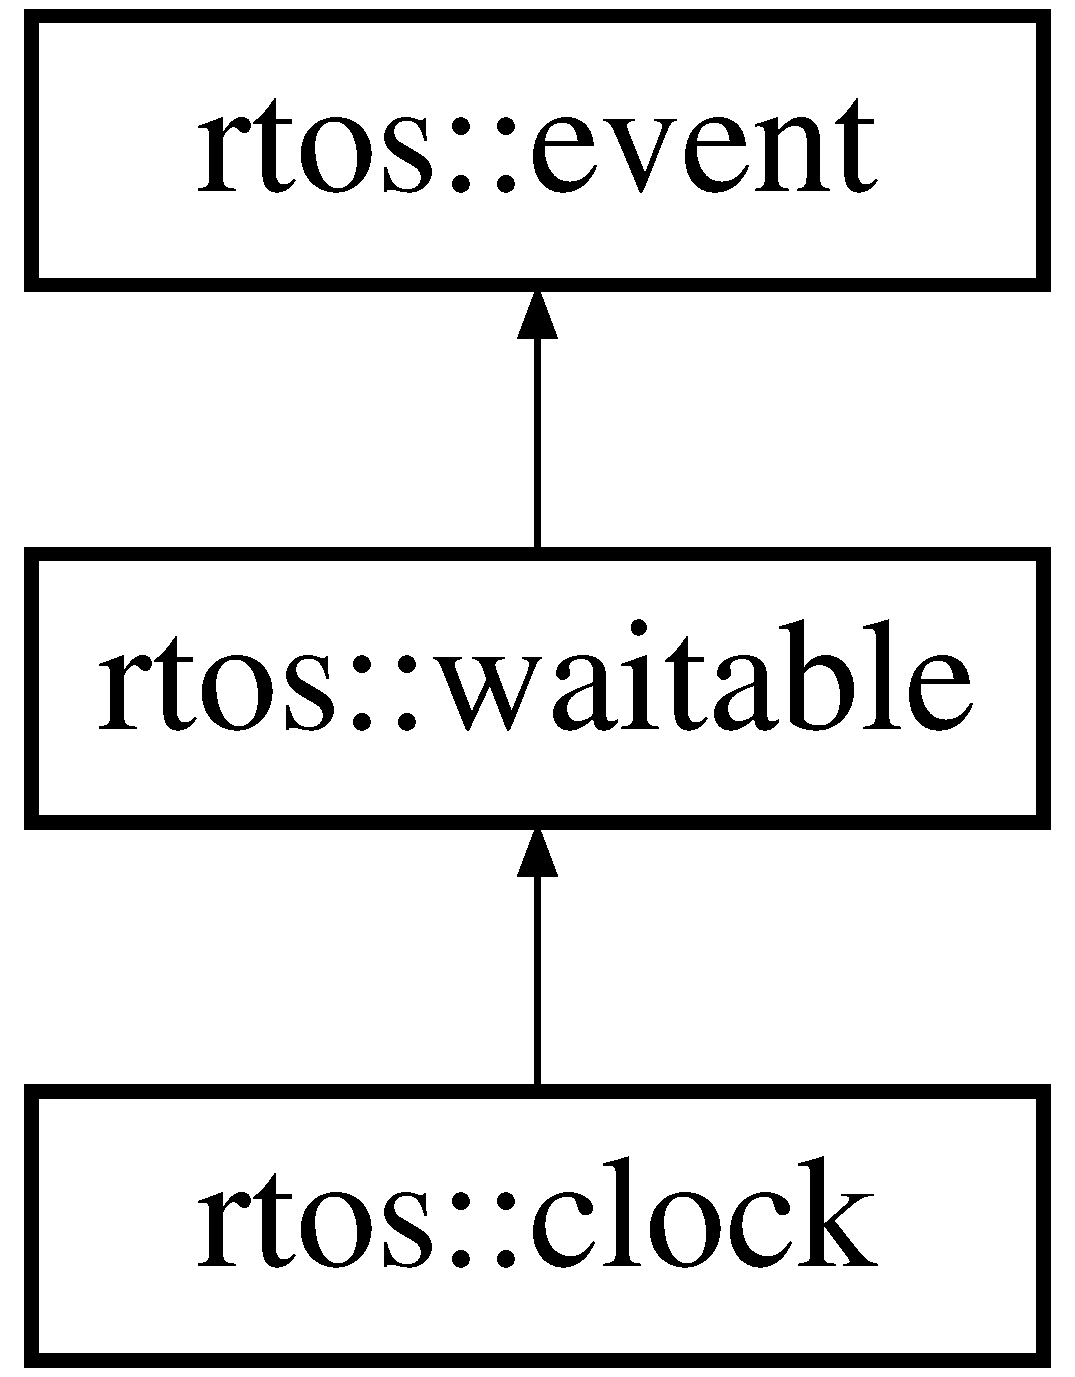
\includegraphics[height=3.000000cm]{classrtos_1_1clock}
\end{center}
\end{figure}
\subsection*{Public Member Functions}
\begin{DoxyCompactItemize}
\item 
\hyperlink{classrtos_1_1clock_a90279f3e878dbe768e2d98e8ab77be11}{clock} (\hyperlink{classrtos_1_1task__base}{task\+\_\+base} $\ast$\hyperlink{classrtos_1_1event_aa83745aabc941145f00386fd63f6b557}{t}, unsigned long int \+\_\+period, const char $\ast$name=\char`\"{}\char`\"{})
\begin{DoxyCompactList}\small\item\em create a clock for task t, specify interval and name \end{DoxyCompactList}\item 
void \hyperlink{classrtos_1_1clock_aa90115db325c074071ae956cb101f046}{clear} (void)
\begin{DoxyCompactList}\small\item\em clear the waitable within the clock \end{DoxyCompactList}\item 
unsigned long int \hyperlink{classrtos_1_1clock_a651c02bc336ba64ac3d2b261f0a31942}{interval} (void)\hypertarget{classrtos_1_1clock_a651c02bc336ba64ac3d2b261f0a31942}{}\label{classrtos_1_1clock_a651c02bc336ba64ac3d2b261f0a31942}

\begin{DoxyCompactList}\small\item\em the interval of the clock \end{DoxyCompactList}\item 
void \hyperlink{classrtos_1_1clock_a2b61cfa27fc686915fa51fc6d7444231}{print} (hwlib\+::ostream \&s, bool header=true) const \hypertarget{classrtos_1_1clock_a2b61cfa27fc686915fa51fc6d7444231}{}\label{classrtos_1_1clock_a2b61cfa27fc686915fa51fc6d7444231}

\begin{DoxyCompactList}\small\item\em print the clock (for debugging) \end{DoxyCompactList}\end{DoxyCompactItemize}
\subsection*{Friends}
\begin{DoxyCompactItemize}
\item 
class {\bfseries rtos}\hypertarget{classrtos_1_1clock_a2a7bcfc34141352757ad672e3ecd099f}{}\label{classrtos_1_1clock_a2a7bcfc34141352757ad672e3ecd099f}

\end{DoxyCompactItemize}
\subsection*{Additional Inherited Members}


\subsection{Detailed Description}
free-\/running clock, ticks at a fixed frequency 

A clock is a waitable which is automatically sets itself at fixed intervals. The interval between these moments is specified when the clock is created. A clock is always running, even when the task to which it belongs is suspended. 

\subsection{Constructor \& Destructor Documentation}
\index{rtos\+::clock@{rtos\+::clock}!clock@{clock}}
\index{clock@{clock}!rtos\+::clock@{rtos\+::clock}}
\subsubsection[{\texorpdfstring{clock(task\+\_\+base $\ast$t, unsigned long int \+\_\+period, const char $\ast$name="""")}{clock(task_base *t, unsigned long int _period, const char *name="")}}]{\setlength{\rightskip}{0pt plus 5cm}rtos\+::clock\+::clock (
\begin{DoxyParamCaption}
\item[{{\bf task\+\_\+base} $\ast$}]{t, }
\item[{unsigned long int}]{\+\_\+period, }
\item[{const char $\ast$}]{name = {\ttfamily \char`\"{}\char`\"{}}}
\end{DoxyParamCaption}
)}\hypertarget{classrtos_1_1clock_a90279f3e878dbe768e2d98e8ab77be11}{}\label{classrtos_1_1clock_a90279f3e878dbe768e2d98e8ab77be11}


create a clock for task t, specify interval and name 

The name is used for debugging and statistics. 

\subsection{Member Function Documentation}
\index{rtos\+::clock@{rtos\+::clock}!clear@{clear}}
\index{clear@{clear}!rtos\+::clock@{rtos\+::clock}}
\subsubsection[{\texorpdfstring{clear(void)}{clear(void)}}]{\setlength{\rightskip}{0pt plus 5cm}void rtos\+::clock\+::clear (
\begin{DoxyParamCaption}
\item[{void}]{}
\end{DoxyParamCaption}
)\hspace{0.3cm}{\ttfamily [inline]}, {\ttfamily [virtual]}}\hypertarget{classrtos_1_1clock_aa90115db325c074071ae956cb101f046}{}\label{classrtos_1_1clock_aa90115db325c074071ae956cb101f046}


clear the waitable within the clock 

Note that this does not stop the clock. 

Reimplemented from \hyperlink{classrtos_1_1waitable_ac4630398f50ba7e661a64bfc491ffa10}{rtos\+::waitable}.



The documentation for this class was generated from the following files\+:\begin{DoxyCompactItemize}
\item 
rtos.\+hpp\item 
rtos.\+cpp\end{DoxyCompactItemize}

\hypertarget{classcoroutine}{}\section{coroutine$<$ N $>$ Class Template Reference}
\label{classcoroutine}\index{coroutine$<$ N $>$@{coroutine$<$ N $>$}}
\subsection*{Public Member Functions}
\begin{DoxyCompactItemize}
\item 
\hyperlink{classcoroutine_a9afea892c919ede99a4882d695cd99ae}{coroutine} (void body(void))
\begin{DoxyCompactList}\small\item\em construct a coroutine from its stack size and main function \end{DoxyCompactList}\end{DoxyCompactItemize}


\subsection{Constructor \& Destructor Documentation}
\index{coroutine@{coroutine}!coroutine@{coroutine}}
\index{coroutine@{coroutine}!coroutine@{coroutine}}
\subsubsection[{\texorpdfstring{coroutine(void body(void))}{coroutine(void body(void))}}]{\setlength{\rightskip}{0pt plus 5cm}template$<$int N$>$ {\bf coroutine}$<$ N $>$\+::{\bf coroutine} (
\begin{DoxyParamCaption}
\item[{void }]{bodyvoid}
\end{DoxyParamCaption}
)\hspace{0.3cm}{\ttfamily [inline]}}\hypertarget{classcoroutine_a9afea892c919ede99a4882d695cd99ae}{}\label{classcoroutine_a9afea892c919ede99a4882d695cd99ae}


construct a coroutine from its stack size and main function 

This constructor creates a coroutine from itsb stack size (this is the template parameter, in bytes, the default is 8K), and a function that is its body. The body function must not return. 

The documentation for this class was generated from the following file\+:\begin{DoxyCompactItemize}
\item 
coroutine.\+hpp\end{DoxyCompactItemize}

\hypertarget{classcoroutine_3_010_01_4}{}\section{coroutine$<$ 0 $>$ Class Template Reference}
\label{classcoroutine_3_010_01_4}\index{coroutine$<$ 0 $>$@{coroutine$<$ 0 $>$}}


coroutine class  




{\ttfamily \#include $<$coroutine.\+hpp$>$}

\subsection*{Public Member Functions}
\begin{DoxyCompactItemize}
\item 
void \hyperlink{classcoroutine_3_010_01_4_ab2afad14fd6145bc0588baec6b8bbe32}{resume} ()
\begin{DoxyCompactList}\small\item\em pass execution to this coroutine \end{DoxyCompactList}\item 
int \hyperlink{classcoroutine_3_010_01_4_af96766f45ce91a5c4e8a05a17f547ebb}{stack\+\_\+free} ()\hypertarget{classcoroutine_3_010_01_4_af96766f45ce91a5c4e8a05a17f547ebb}{}\label{classcoroutine_3_010_01_4_af96766f45ce91a5c4e8a05a17f547ebb}

\begin{DoxyCompactList}\small\item\em return number of unused stack bytes \end{DoxyCompactList}\item 
int \hyperlink{classcoroutine_3_010_01_4_a38b24aa521d80e98e2245ca7956510cb}{stack\+\_\+used} ()\hypertarget{classcoroutine_3_010_01_4_a38b24aa521d80e98e2245ca7956510cb}{}\label{classcoroutine_3_010_01_4_a38b24aa521d80e98e2245ca7956510cb}

\begin{DoxyCompactList}\small\item\em return number of used stack bytes \end{DoxyCompactList}\end{DoxyCompactItemize}
\subsection*{Static Public Member Functions}
\begin{DoxyCompactItemize}
\item 
static void \hyperlink{classcoroutine_3_010_01_4_ac7552b0b1e00a303967255a49b923edb}{resume\+\_\+main} ()
\begin{DoxyCompactList}\small\item\em pass execution to the main \textquotesingle{}coroutine\textquotesingle{} \end{DoxyCompactList}\end{DoxyCompactItemize}
\subsection*{Public Attributes}
\begin{DoxyCompactItemize}
\item 
const int \hyperlink{classcoroutine_3_010_01_4_a3a60f49f800cd809f30cb08d10791319}{stack\+\_\+size}\hypertarget{classcoroutine_3_010_01_4_a3a60f49f800cd809f30cb08d10791319}{}\label{classcoroutine_3_010_01_4_a3a60f49f800cd809f30cb08d10791319}

\begin{DoxyCompactList}\small\item\em the size (in bytes) of the stack allocated for this coroutine \end{DoxyCompactList}\end{DoxyCompactItemize}
\subsection*{Protected Member Functions}
\begin{DoxyCompactItemize}
\item 
{\bfseries coroutine} (void body(void), int $\ast$stack, int int\+\_\+stack\+\_\+size)\hypertarget{classcoroutine_3_010_01_4_a0b84949051013d4b0285ad61c22ed5b8}{}\label{classcoroutine_3_010_01_4_a0b84949051013d4b0285ad61c22ed5b8}

\end{DoxyCompactItemize}


\subsection{Detailed Description}
\subsubsection*{template$<$$>$\\*
class coroutine$<$ 0 $>$}

coroutine class 

This class implements a coroutine\+: an independent thread of execution that can pass execution to another coroutine by calling \hyperlink{classcoroutine_3_010_01_4_ab2afad14fd6145bc0588baec6b8bbe32}{resume()} on that coroutine. This can be used as the basis for a co-\/operative multithreading system. 

\subsection{Member Function Documentation}
\index{coroutine$<$ 0 $>$@{coroutine$<$ 0 $>$}!resume@{resume}}
\index{resume@{resume}!coroutine$<$ 0 $>$@{coroutine$<$ 0 $>$}}
\subsubsection[{\texorpdfstring{resume()}{resume()}}]{\setlength{\rightskip}{0pt plus 5cm}void {\bf coroutine}$<$ 0 $>$\+::resume (
\begin{DoxyParamCaption}
{}
\end{DoxyParamCaption}
)\hspace{0.3cm}{\ttfamily [inline]}}\hypertarget{classcoroutine_3_010_01_4_ab2afad14fd6145bc0588baec6b8bbe32}{}\label{classcoroutine_3_010_01_4_ab2afad14fd6145bc0588baec6b8bbe32}


pass execution to this coroutine 

Call this function on a coroutine object to activate (start or resume) execution of that coroutine. The current coroutine is suspended. Execution of a coroutine starts by execution its body function (the function that was passed to its constructor). Resuming a coroutine continues execution after the \hyperlink{classcoroutine_3_010_01_4_ab2afad14fd6145bc0588baec6b8bbe32}{resume()} call that suspended it.

Initially, the main is executing, so it must issue the first \hyperlink{classcoroutine_3_010_01_4_ab2afad14fd6145bc0588baec6b8bbe32}{resume()} call on a coroutine. A coroutine body function must not return. \index{coroutine$<$ 0 $>$@{coroutine$<$ 0 $>$}!resume\+\_\+main@{resume\+\_\+main}}
\index{resume\+\_\+main@{resume\+\_\+main}!coroutine$<$ 0 $>$@{coroutine$<$ 0 $>$}}
\subsubsection[{\texorpdfstring{resume\+\_\+main()}{resume_main()}}]{\setlength{\rightskip}{0pt plus 5cm}static void {\bf coroutine}$<$ 0 $>$\+::resume\+\_\+main (
\begin{DoxyParamCaption}
{}
\end{DoxyParamCaption}
)\hspace{0.3cm}{\ttfamily [inline]}, {\ttfamily [static]}}\hypertarget{classcoroutine_3_010_01_4_ac7552b0b1e00a303967255a49b923edb}{}\label{classcoroutine_3_010_01_4_ac7552b0b1e00a303967255a49b923edb}


pass execution to the main \textquotesingle{}coroutine\textquotesingle{} 

Call this function to re-\/activate (resume) the main \textquotesingle{}coroutine\textquotesingle{}. The current coroutine is suspended. 

The documentation for this class was generated from the following file\+:\begin{DoxyCompactItemize}
\item 
coroutine.\+hpp\end{DoxyCompactItemize}

\hypertarget{classcoroutine__context}{}\section{coroutine\+\_\+context Class Reference}
\label{classcoroutine__context}\index{coroutine\+\_\+context@{coroutine\+\_\+context}}
\subsection*{Friends}
\begin{DoxyCompactItemize}
\item 
class {\bfseries coroutine$<$ 0 $>$}\hypertarget{classcoroutine__context_a874ca9b5dbeb1f6d90f61bc87474e164}{}\label{classcoroutine__context_a874ca9b5dbeb1f6d90f61bc87474e164}

\end{DoxyCompactItemize}


The documentation for this class was generated from the following files\+:\begin{DoxyCompactItemize}
\item 
coroutine.\+hpp\item 
coroutine.\+cpp\end{DoxyCompactItemize}

\hypertarget{classrtos_1_1event}{}\section{rtos\+:\+:event Class Reference}
\label{classrtos_1_1event}\index{rtos\+::event@{rtos\+::event}}


set of things that can happen, or a thing that has happened  




{\ttfamily \#include $<$rtos.\+hpp$>$}

Inheritance diagram for rtos\+:\+:event\+:\begin{figure}[H]
\begin{center}
\leavevmode
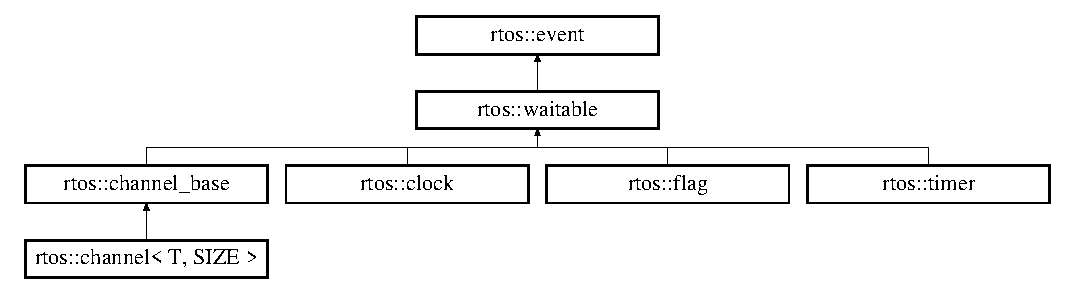
\includegraphics[height=3.500000cm]{classrtos_1_1event}
\end{center}
\end{figure}
\subsection*{Public Member Functions}
\begin{DoxyCompactItemize}
\item 
void \hyperlink{classrtos_1_1event_a9f335615e161cabbc504878ef03c3bf3}{print} (hwlib\+::ostream \&s) const \hypertarget{classrtos_1_1event_a9f335615e161cabbc504878ef03c3bf3}{}\label{classrtos_1_1event_a9f335615e161cabbc504878ef03c3bf3}

\begin{DoxyCompactList}\small\item\em prints an event, for debugging only \end{DoxyCompactList}\item 
bool \hyperlink{classrtos_1_1event_a1c0523abc492cb47b4ef37a762ddc442}{operator==} (const \hyperlink{classrtos_1_1event}{event} \&rhs) const \hypertarget{classrtos_1_1event_a1c0523abc492cb47b4ef37a762ddc442}{}\label{classrtos_1_1event_a1c0523abc492cb47b4ef37a762ddc442}

\begin{DoxyCompactList}\small\item\em report wether two events are the same \end{DoxyCompactList}\item 
bool \hyperlink{classrtos_1_1event_a6a8c2497baaddf6c19d045578413f966}{operator==} (const \hyperlink{classrtos_1_1waitable}{waitable} \&rhs) const \hypertarget{classrtos_1_1event_a6a8c2497baaddf6c19d045578413f966}{}\label{classrtos_1_1event_a6a8c2497baaddf6c19d045578413f966}

\begin{DoxyCompactList}\small\item\em report whether an event corresponds to a waitable \end{DoxyCompactList}\item 
bool \hyperlink{classrtos_1_1event_ac90eda8c24bf2915de25166bd2b1411f}{operator!=} (const \hyperlink{classrtos_1_1event}{event} \&rhs) const \hypertarget{classrtos_1_1event_ac90eda8c24bf2915de25166bd2b1411f}{}\label{classrtos_1_1event_ac90eda8c24bf2915de25166bd2b1411f}

\begin{DoxyCompactList}\small\item\em report wether two events are not the same \end{DoxyCompactList}\item 
bool \hyperlink{classrtos_1_1event_ae3dcd2feb206d88ecf03920d60f48a27}{operator!=} (const \hyperlink{classrtos_1_1waitable}{waitable} \&rhs) const \hypertarget{classrtos_1_1event_ae3dcd2feb206d88ecf03920d60f48a27}{}\label{classrtos_1_1event_ae3dcd2feb206d88ecf03920d60f48a27}

\begin{DoxyCompactList}\small\item\em report whether an event does not correspond to a waitable \end{DoxyCompactList}\item 
\hyperlink{classrtos_1_1event}{event} \hyperlink{classrtos_1_1event_af75155ce72b01bd2927a411643ddae89}{operator+} (const \hyperlink{classrtos_1_1event}{event} \&rhs) const 
\begin{DoxyCompactList}\small\item\em add two waitables, result can be used in a wait() call \end{DoxyCompactList}\end{DoxyCompactItemize}
\subsection*{Protected Member Functions}
\begin{DoxyCompactItemize}
\item 
\hyperlink{classrtos_1_1event_a6cbf4e72e1d4ab312b3901ed54f4d48e}{event} (\hyperlink{classrtos_1_1task__base}{task\+\_\+base} $\ast$\hyperlink{classrtos_1_1event_aa83745aabc941145f00386fd63f6b557}{t}, unsigned int \hyperlink{classrtos_1_1event_aa6e6f66f74b4f1523e456d34dd7a1704}{mask})\hypertarget{classrtos_1_1event_a6cbf4e72e1d4ab312b3901ed54f4d48e}{}\label{classrtos_1_1event_a6cbf4e72e1d4ab312b3901ed54f4d48e}

\begin{DoxyCompactList}\small\item\em constructor, used by concrete events \end{DoxyCompactList}\end{DoxyCompactItemize}
\subsection*{Protected Attributes}
\begin{DoxyCompactItemize}
\item 
\hyperlink{classrtos_1_1task__base}{task\+\_\+base} $\ast$ \hyperlink{classrtos_1_1event_aa83745aabc941145f00386fd63f6b557}{t}\hypertarget{classrtos_1_1event_aa83745aabc941145f00386fd63f6b557}{}\label{classrtos_1_1event_aa83745aabc941145f00386fd63f6b557}

\begin{DoxyCompactList}\small\item\em the owner task \end{DoxyCompactList}\item 
unsigned int \hyperlink{classrtos_1_1event_aa6e6f66f74b4f1523e456d34dd7a1704}{mask}
\begin{DoxyCompactList}\small\item\em the mask of this event, one bit is set \end{DoxyCompactList}\end{DoxyCompactItemize}
\subsection*{Friends}
\begin{DoxyCompactItemize}
\item 
class {\bfseries waitable\+\_\+set}\hypertarget{classrtos_1_1event_a0ee29d8961a0b67cea2c3fa76da116da}{}\label{classrtos_1_1event_a0ee29d8961a0b67cea2c3fa76da116da}

\end{DoxyCompactItemize}


\subsection{Detailed Description}
set of things that can happen, or a thing that has happened 

An event
\begin{DoxyItemize}
\item is the result of adding waitables
\item is accepted as argument to wait()
\item is returned by wait()
\item can be compared to a waitable
\end{DoxyItemize}

The \hyperlink{classrtos_1_1task__base_a2590ba76480cecaff66282516fbeb1bb}{task\+::wait()} calls return an event. Such an event can be compared to a waitable. The result is true if and only if the waitable caused the event.

Events are the only R\+T\+OS objects that can be destroyed (without causing an error). 

\subsection{Member Function Documentation}
\index{rtos\+::event@{rtos\+::event}!operator+@{operator+}}
\index{operator+@{operator+}!rtos\+::event@{rtos\+::event}}
\subsubsection[{\texorpdfstring{operator+(const event \&rhs) const }{operator+(const event &rhs) const }}]{\setlength{\rightskip}{0pt plus 5cm}{\bf rtos\+::event} rtos\+::event\+::operator+ (
\begin{DoxyParamCaption}
\item[{const {\bf event} \&}]{rhs}
\end{DoxyParamCaption}
) const}\hypertarget{classrtos_1_1event_af75155ce72b01bd2927a411643ddae89}{}\label{classrtos_1_1event_af75155ce72b01bd2927a411643ddae89}


add two waitables, result can be used in a wait() call 

Waitables can be added (operator+) to construct a \textquotesingle{}set of waitables\textquotesingle{} as argument to a \hyperlink{classrtos_1_1task__base_a2590ba76480cecaff66282516fbeb1bb}{task\+::wait()} call. 

\subsection{Member Data Documentation}
\index{rtos\+::event@{rtos\+::event}!mask@{mask}}
\index{mask@{mask}!rtos\+::event@{rtos\+::event}}
\subsubsection[{\texorpdfstring{mask}{mask}}]{\setlength{\rightskip}{0pt plus 5cm}unsigned int rtos\+::event\+::mask\hspace{0.3cm}{\ttfamily [protected]}}\hypertarget{classrtos_1_1event_aa6e6f66f74b4f1523e456d34dd7a1704}{}\label{classrtos_1_1event_aa6e6f66f74b4f1523e456d34dd7a1704}


the mask of this event, one bit is set 

The bit that is set is unique among the events owned by a task. 

The documentation for this class was generated from the following files\+:\begin{DoxyCompactItemize}
\item 
rtos.\+hpp\item 
rtos.\+cpp\end{DoxyCompactItemize}

\hypertarget{classrtos_1_1flag}{}\section{rtos\+:\+:flag Class Reference}
\label{classrtos_1_1flag}\index{rtos\+::flag@{rtos\+::flag}}


basic synchronisation mechanism.  




{\ttfamily \#include $<$rtos.\+hpp$>$}

Inheritance diagram for rtos\+:\+:flag\+:\begin{figure}[H]
\begin{center}
\leavevmode
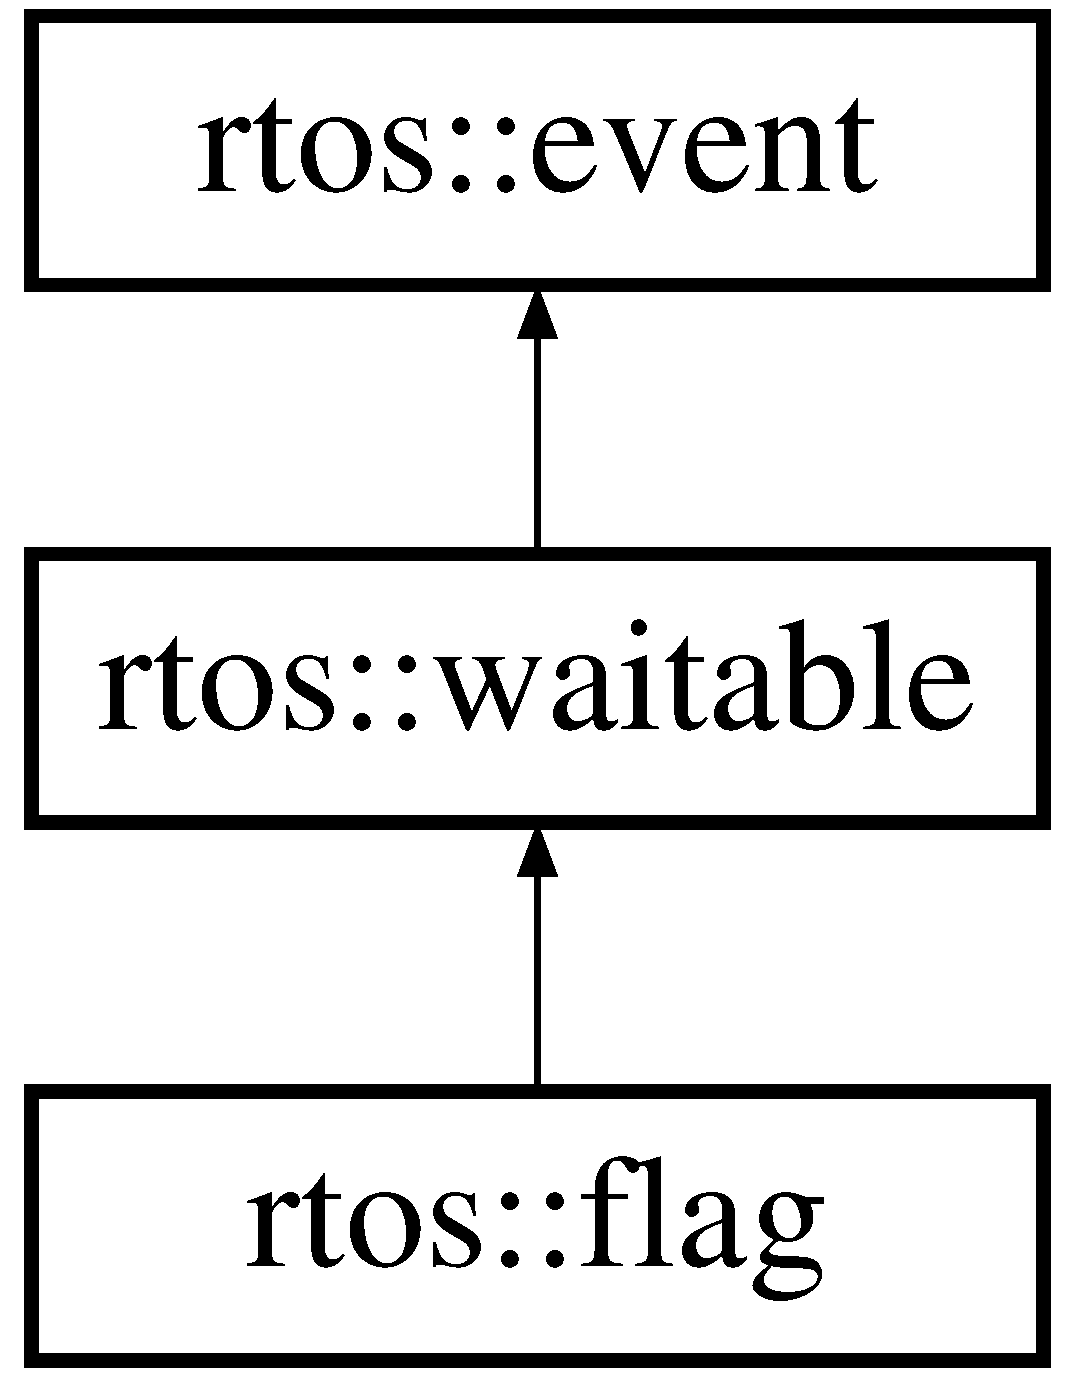
\includegraphics[height=3.000000cm]{classrtos_1_1flag}
\end{center}
\end{figure}
\subsection*{Public Member Functions}
\begin{DoxyCompactItemize}
\item 
\hyperlink{classrtos_1_1flag_af4fa671e37438103a9f12f7e0c87a6b2}{flag} (\hyperlink{classrtos_1_1task__base}{task\+\_\+base} $\ast$\hyperlink{classrtos_1_1event_aa83745aabc941145f00386fd63f6b557}{t}, const char $\ast$name=\char`\"{}\char`\"{})
\begin{DoxyCompactList}\small\item\em constructor, specify onwer and name \end{DoxyCompactList}\item 
void \hyperlink{classrtos_1_1flag_a7372dff631de89809f25edef544ff884}{set} (void)
\begin{DoxyCompactList}\small\item\em sets the flag \end{DoxyCompactList}\item 
void \hyperlink{classrtos_1_1flag_a49932267b755b23e8325849527330c2f}{print} (hwlib\+::ostream \&s, bool header=true) const \hypertarget{classrtos_1_1flag_a49932267b755b23e8325849527330c2f}{}\label{classrtos_1_1flag_a49932267b755b23e8325849527330c2f}

\begin{DoxyCompactList}\small\item\em prints flag infomation (for debugging) \end{DoxyCompactList}\end{DoxyCompactItemize}
\subsection*{Friends}
\begin{DoxyCompactItemize}
\item 
class {\bfseries rtos}\hypertarget{classrtos_1_1flag_a2a7bcfc34141352757ad672e3ecd099f}{}\label{classrtos_1_1flag_a2a7bcfc34141352757ad672e3ecd099f}

\end{DoxyCompactItemize}
\subsection*{Additional Inherited Members}


\subsection{Detailed Description}
basic synchronisation mechanism. 

The basic synchronization mechanism is the (event) flag. Like all waitables, a flag is created for a particular task. A flag is set by a \hyperlink{classrtos_1_1flag_a7372dff631de89809f25edef544ff884}{flag\+::set()} call (or the task\+::set( flag) call, which has the same effect). Like all waitables, when a task is waiting for a flag (using a \hyperlink{classrtos_1_1task__base_a2590ba76480cecaff66282516fbeb1bb}{task\+::wait} call) and that flag becomes set, the wait call will clear the flag, and return an event that compares equal to the flag. Note that a flag does not count\+: setting a flag that is already set has no effect on the flag.

A flag must be created for a specific task. The normal place to do this is in the task\textquotesingle{}s creator. An flag is initially cleared.

The example below shows a led\+\_\+task that responds to two event flags. The shift flag will cause it to shift the pattern on the L\+E\+Ds one position to the left, while the invert flag will cause it to invert the pattern. Two addional tasks do notghing but set these flags at fixed intervals. The result is a sort of one-\/direction Kitt display, which will occasionally flip polarity. Note that in this example the wait call excplicitly mentions the flags it waits for. 

\subsection{Constructor \& Destructor Documentation}
\index{rtos\+::flag@{rtos\+::flag}!flag@{flag}}
\index{flag@{flag}!rtos\+::flag@{rtos\+::flag}}
\subsubsection[{\texorpdfstring{flag(task\+\_\+base $\ast$t, const char $\ast$name="""")}{flag(task_base *t, const char *name="")}}]{\setlength{\rightskip}{0pt plus 5cm}rtos\+::flag\+::flag (
\begin{DoxyParamCaption}
\item[{{\bf task\+\_\+base} $\ast$}]{t, }
\item[{const char $\ast$}]{name = {\ttfamily \char`\"{}\char`\"{}}}
\end{DoxyParamCaption}
)}\hypertarget{classrtos_1_1flag_af4fa671e37438103a9f12f7e0c87a6b2}{}\label{classrtos_1_1flag_af4fa671e37438103a9f12f7e0c87a6b2}


constructor, specify onwer and name 

This call creates a timer for task t. The name is used for debugging and statistics. 

\subsection{Member Function Documentation}
\index{rtos\+::flag@{rtos\+::flag}!set@{set}}
\index{set@{set}!rtos\+::flag@{rtos\+::flag}}
\subsubsection[{\texorpdfstring{set(void)}{set(void)}}]{\setlength{\rightskip}{0pt plus 5cm}void rtos\+::flag\+::set (
\begin{DoxyParamCaption}
\item[{void}]{}
\end{DoxyParamCaption}
)}\hypertarget{classrtos_1_1flag_a7372dff631de89809f25edef544ff884}{}\label{classrtos_1_1flag_a7372dff631de89809f25edef544ff884}


sets the flag 

Setting a flag causes the task that waits for this flag to be awakened. 

The documentation for this class was generated from the following files\+:\begin{DoxyCompactItemize}
\item 
rtos.\+hpp\item 
rtos.\+cpp\end{DoxyCompactItemize}

\hypertarget{classrtos_1_1mailbox}{}\section{rtos\+:\+:mailbox$<$ T $>$ Class Template Reference}
\label{classrtos_1_1mailbox}\index{rtos\+::mailbox$<$ T $>$@{rtos\+::mailbox$<$ T $>$}}


Synchronously handing over of a data item.  




{\ttfamily \#include $<$rtos.\+hpp$>$}

Inheritance diagram for rtos\+:\+:mailbox$<$ T $>$\+:\begin{figure}[H]
\begin{center}
\leavevmode
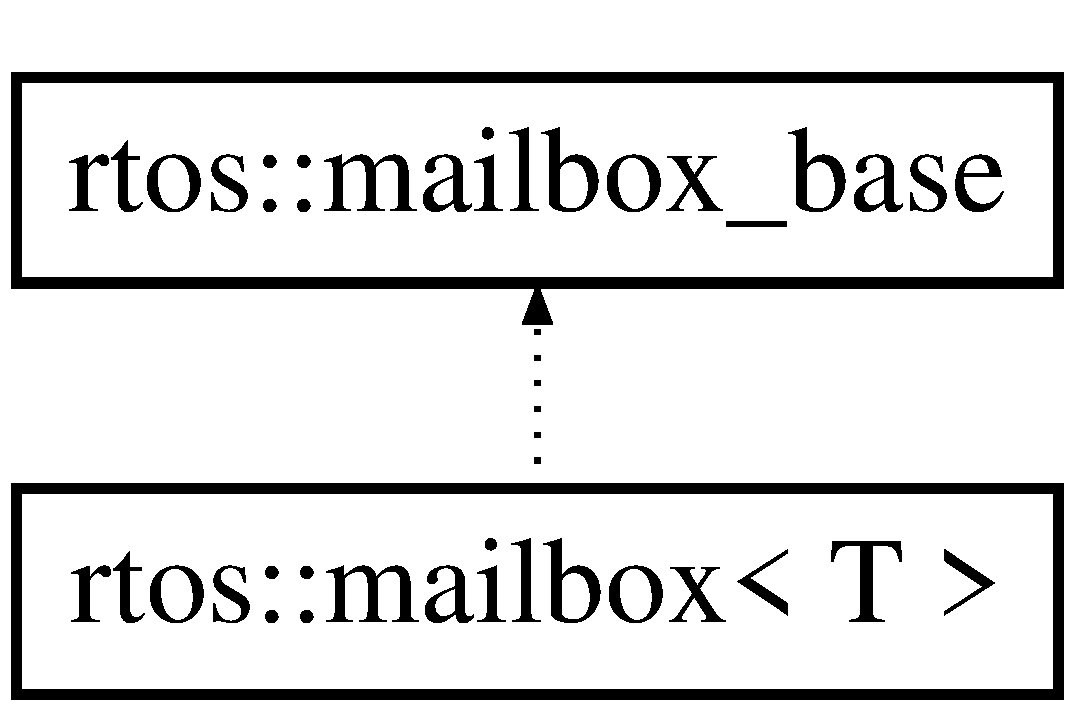
\includegraphics[height=2.000000cm]{classrtos_1_1mailbox}
\end{center}
\end{figure}
\subsection*{Public Member Functions}
\begin{DoxyCompactItemize}
\item 
\hyperlink{classrtos_1_1mailbox_a31d61fcc4b21f6450ffc55f7de1da968}{mailbox} (const char $\ast$name=\char`\"{}\char`\"{})
\begin{DoxyCompactList}\small\item\em constructor, specify mailbox name \end{DoxyCompactList}\item 
void \hyperlink{classrtos_1_1mailbox_aa49a194170b9a498982c7867462e99d0}{write} (const T item)
\item 
T \hyperlink{classrtos_1_1mailbox_aba12a2a7ff395526f88eb9014e26604a}{read} (void)
\begin{DoxyCompactList}\small\item\em read a value from the mailbox \end{DoxyCompactList}\end{DoxyCompactItemize}


\subsection{Detailed Description}
\subsubsection*{template$<$class T$>$\\*
class rtos\+::mailbox$<$ T $>$}

Synchronously handing over of a data item. 

A mailbox is a template class synchronization mechanism. A single value can be written to the mailbox. Another task can read the value from the mailbox. The read and write calls wait on each other before they are allowed to proceed.

A mailbox is not created for a particular task, and it is not a waitable.

Initially a mailbox is empty. The \hyperlink{classrtos_1_1mailbox_aa49a194170b9a498982c7867462e99d0}{write()} operation writes to the mailbox, and, if present, unblocks a reading task and returns, otherwise the writing task is blocked. The \hyperlink{classrtos_1_1mailbox_aba12a2a7ff395526f88eb9014e26604a}{read()} operation blocks the calling task until there is a value in the mailbox. Then it reads the value, unblocks the task that wrote to the mailbox, and returns. 

\subsection{Constructor \& Destructor Documentation}
\index{rtos\+::mailbox@{rtos\+::mailbox}!mailbox@{mailbox}}
\index{mailbox@{mailbox}!rtos\+::mailbox@{rtos\+::mailbox}}
\subsubsection[{\texorpdfstring{mailbox(const char $\ast$name="""")}{mailbox(const char *name="")}}]{\setlength{\rightskip}{0pt plus 5cm}template$<$class T $>$ {\bf rtos\+::mailbox}$<$ T $>$\+::{\bf mailbox} (
\begin{DoxyParamCaption}
\item[{const char $\ast$}]{name = {\ttfamily \char`\"{}\char`\"{}}}
\end{DoxyParamCaption}
)\hspace{0.3cm}{\ttfamily [inline]}}\hypertarget{classrtos_1_1mailbox_a31d61fcc4b21f6450ffc55f7de1da968}{}\label{classrtos_1_1mailbox_a31d61fcc4b21f6450ffc55f7de1da968}


constructor, specify mailbox name 

Create a mailbox. The mailbox is initially empty. The template argument T must be a class that has a non-\/arguments constructor and supports assignment. 

\subsection{Member Function Documentation}
\index{rtos\+::mailbox@{rtos\+::mailbox}!read@{read}}
\index{read@{read}!rtos\+::mailbox@{rtos\+::mailbox}}
\subsubsection[{\texorpdfstring{read(void)}{read(void)}}]{\setlength{\rightskip}{0pt plus 5cm}template$<$class T $>$ T {\bf rtos\+::mailbox}$<$ T $>$\+::read (
\begin{DoxyParamCaption}
\item[{void}]{}
\end{DoxyParamCaption}
)\hspace{0.3cm}{\ttfamily [inline]}}\hypertarget{classrtos_1_1mailbox_aba12a2a7ff395526f88eb9014e26604a}{}\label{classrtos_1_1mailbox_aba12a2a7ff395526f88eb9014e26604a}


read a value from the mailbox 

If a writing tasks is waiting for the mailbox it is unblocked and the reader gets the data. Otherwise the current task is blocked until it is released by a writer. \index{rtos\+::mailbox@{rtos\+::mailbox}!write@{write}}
\index{write@{write}!rtos\+::mailbox@{rtos\+::mailbox}}
\subsubsection[{\texorpdfstring{write(const T item)}{write(const T item)}}]{\setlength{\rightskip}{0pt plus 5cm}template$<$class T $>$ void {\bf rtos\+::mailbox}$<$ T $>$\+::write (
\begin{DoxyParamCaption}
\item[{const T}]{item}
\end{DoxyParamCaption}
)\hspace{0.3cm}{\ttfamily [inline]}}\hypertarget{classrtos_1_1mailbox_aa49a194170b9a498982c7867462e99d0}{}\label{classrtos_1_1mailbox_aa49a194170b9a498982c7867462e99d0}
write an item into the mailbox

The current (writing) task stores an item in the mailbox. If a client (reader) is waiting, it is unblocked. Otherwise the task waits (is blocked) until a reading task has read the item. 

The documentation for this class was generated from the following file\+:\begin{DoxyCompactItemize}
\item 
rtos.\+hpp\end{DoxyCompactItemize}

\hypertarget{classrtos_1_1mailbox__base}{}\section{rtos\+:\+:mailbox\+\_\+base Class Reference}
\label{classrtos_1_1mailbox__base}\index{rtos\+::mailbox\+\_\+base@{rtos\+::mailbox\+\_\+base}}


rtos private implementation class  




{\ttfamily \#include $<$rtos.\+hpp$>$}

Inheritance diagram for rtos\+:\+:mailbox\+\_\+base\+:\begin{figure}[H]
\begin{center}
\leavevmode
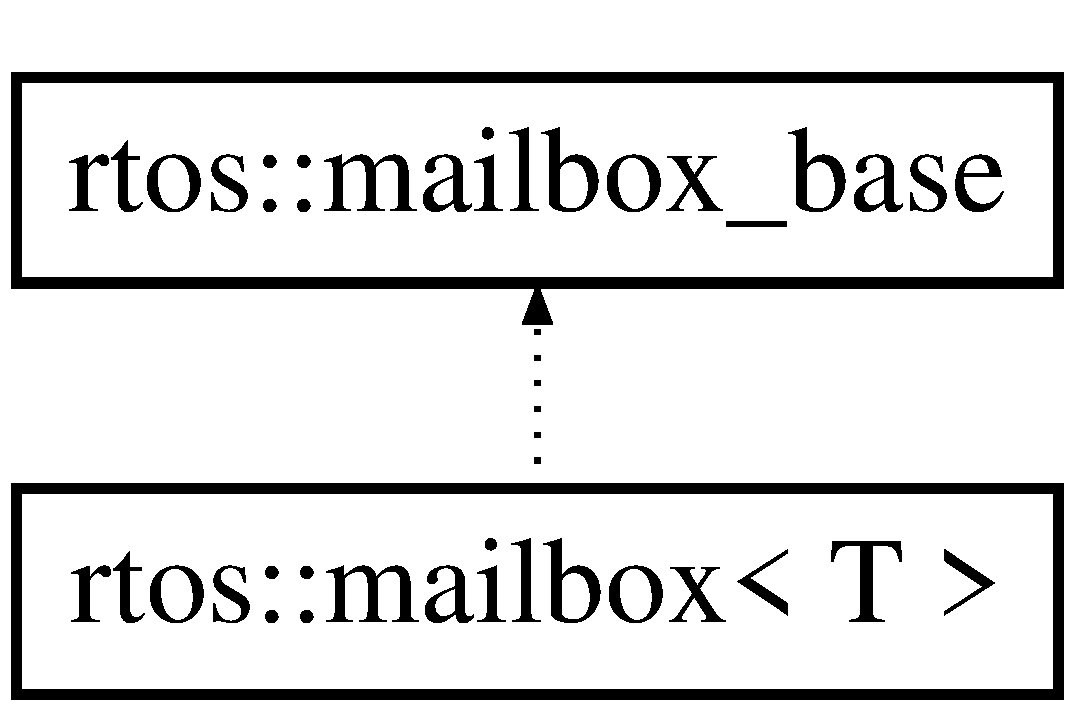
\includegraphics[height=2.000000cm]{classrtos_1_1mailbox__base}
\end{center}
\end{figure}
\subsection*{Public Member Functions}
\begin{DoxyCompactItemize}
\item 
{\bfseries mailbox\+\_\+base} (const char $\ast$name)\hypertarget{classrtos_1_1mailbox__base_a647b58f572b4e387afe926eb4aa1592d}{}\label{classrtos_1_1mailbox__base_a647b58f572b4e387afe926eb4aa1592d}

\item 
void {\bfseries print} (hwlib\+::ostream \&s, bool header=true) const \hypertarget{classrtos_1_1mailbox__base_a4d45169c0f5dd6a18cc1c6218d248126}{}\label{classrtos_1_1mailbox__base_a4d45169c0f5dd6a18cc1c6218d248126}

\end{DoxyCompactItemize}
\subsection*{Public Attributes}
\begin{DoxyCompactItemize}
\item 
\hyperlink{classrtos_1_1task__base}{task\+\_\+base} $\ast$ {\bfseries writer}\hypertarget{classrtos_1_1mailbox__base_ab6916cbb6931c728a256cb59b86a19ad}{}\label{classrtos_1_1mailbox__base_ab6916cbb6931c728a256cb59b86a19ad}

\item 
\hyperlink{classrtos_1_1task__base}{task\+\_\+base} $\ast$ {\bfseries reader}\hypertarget{classrtos_1_1mailbox__base_aacbf86c2dc3d6a3cb19ab3b32a86ead8}{}\label{classrtos_1_1mailbox__base_aacbf86c2dc3d6a3cb19ab3b32a86ead8}

\item 
const char $\ast$ {\bfseries mailbox\+\_\+name}\hypertarget{classrtos_1_1mailbox__base_ad6c99f06c6ae8662b40090040e51f6f5}{}\label{classrtos_1_1mailbox__base_ad6c99f06c6ae8662b40090040e51f6f5}

\item 
unsigned int {\bfseries writes}\hypertarget{classrtos_1_1mailbox__base_a5350e3d0a6d0969c917a630a8255f9f6}{}\label{classrtos_1_1mailbox__base_a5350e3d0a6d0969c917a630a8255f9f6}

\item 
unsigned int {\bfseries reads}\hypertarget{classrtos_1_1mailbox__base_a7d7437c03cca4719cc0c29212c0fc52f}{}\label{classrtos_1_1mailbox__base_a7d7437c03cca4719cc0c29212c0fc52f}

\item 
\hyperlink{classrtos_1_1mailbox__base}{mailbox\+\_\+base} $\ast$ {\bfseries next\+\_\+mailbox}\hypertarget{classrtos_1_1mailbox__base_a3a47e8e62c65ae5f4a0fef12d1bce40b}{}\label{classrtos_1_1mailbox__base_a3a47e8e62c65ae5f4a0fef12d1bce40b}

\end{DoxyCompactItemize}


\subsection{Detailed Description}
rtos private implementation class 

The documentation for this class was generated from the following files\+:\begin{DoxyCompactItemize}
\item 
rtos.\+hpp\item 
rtos.\+cpp\end{DoxyCompactItemize}

\hypertarget{classrtos_1_1mutex}{}\section{rtos\+:\+:mutex Class Reference}
\label{classrtos_1_1mutex}\index{rtos\+::mutex@{rtos\+::mutex}}


mutual execlusion semaphore  




{\ttfamily \#include $<$rtos.\+hpp$>$}

\subsection*{Public Member Functions}
\begin{DoxyCompactItemize}
\item 
\hyperlink{classrtos_1_1mutex_ac406598aa3b34c199c6d4914de392180}{mutex} (const char $\ast$name=\char`\"{}\char`\"{})
\begin{DoxyCompactList}\small\item\em constructor, specify the name \end{DoxyCompactList}\item 
\hyperlink{classrtos_1_1mutex_a6c0644985543ff72112560edc8d70bb0}{$\sim$mutex} (void)
\begin{DoxyCompactList}\small\item\em generates an error \end{DoxyCompactList}\item 
void \hyperlink{classrtos_1_1mutex_a43b6d7a55176945f59598f825a5acd65}{print} (hwlib\+::ostream \&stream, bool header=true) const \hypertarget{classrtos_1_1mutex_a43b6d7a55176945f59598f825a5acd65}{}\label{classrtos_1_1mutex_a43b6d7a55176945f59598f825a5acd65}

\begin{DoxyCompactList}\small\item\em prints a mutex, for debugging only. \end{DoxyCompactList}\item 
void \hyperlink{classrtos_1_1mutex_af005eb2964192bbdf1a444eab11eb683}{wait} (void)
\item 
void \hyperlink{classrtos_1_1mutex_ad57303013f03da5856e54f331323dc5d}{signal} (void)
\begin{DoxyCompactList}\small\item\em release the mutex \end{DoxyCompactList}\end{DoxyCompactItemize}
\subsection*{Friends}
\begin{DoxyCompactItemize}
\item 
class {\bfseries rtos}\hypertarget{classrtos_1_1mutex_a2a7bcfc34141352757ad672e3ecd099f}{}\label{classrtos_1_1mutex_a2a7bcfc34141352757ad672e3ecd099f}

\end{DoxyCompactItemize}


\subsection{Detailed Description}
mutual execlusion semaphore 

A mutex (mutual exclusion semaphore) is a synchronization mechanism that is used to give a task exclusive access to some resource\+: the task can execute a sequence of statements, being sure that no other task is accessing the same resource.

A typical use is to protect a resource (for instance global data) that should be used by only one task at a time, so it can update it and leave it in a consistent state.

A mutex is not created for a particular task, and it is not a waitable.

Initially a mutex is free. The \hyperlink{classrtos_1_1mutex_af005eb2964192bbdf1a444eab11eb683}{mutex\+::wait()} operation blocks the task until the mutex is free, and then claims the mutex for the executing task. The \hyperlink{classrtos_1_1mutex_ad57303013f03da5856e54f331323dc5d}{mutex\+::signal()} operation frees the mutex again. It is an error to call \hyperlink{classrtos_1_1mutex_ad57303013f03da5856e54f331323dc5d}{mutex\+::signal} on a mutex that is not currently owned by the executing task. 

\subsection{Constructor \& Destructor Documentation}
\index{rtos\+::mutex@{rtos\+::mutex}!mutex@{mutex}}
\index{mutex@{mutex}!rtos\+::mutex@{rtos\+::mutex}}
\subsubsection[{\texorpdfstring{mutex(const char $\ast$name="""")}{mutex(const char *name="")}}]{\setlength{\rightskip}{0pt plus 5cm}rtos\+::mutex\+::mutex (
\begin{DoxyParamCaption}
\item[{const char $\ast$}]{name = {\ttfamily \char`\"{}\char`\"{}}}
\end{DoxyParamCaption}
)}\hypertarget{classrtos_1_1mutex_ac406598aa3b34c199c6d4914de392180}{}\label{classrtos_1_1mutex_ac406598aa3b34c199c6d4914de392180}


constructor, specify the name 

The name is used for debugging only. \index{rtos\+::mutex@{rtos\+::mutex}!````~mutex@{$\sim$mutex}}
\index{````~mutex@{$\sim$mutex}!rtos\+::mutex@{rtos\+::mutex}}
\subsubsection[{\texorpdfstring{$\sim$mutex(void)}{~mutex(void)}}]{\setlength{\rightskip}{0pt plus 5cm}rtos\+::mutex\+::$\sim$mutex (
\begin{DoxyParamCaption}
\item[{void}]{}
\end{DoxyParamCaption}
)}\hypertarget{classrtos_1_1mutex_a6c0644985543ff72112560edc8d70bb0}{}\label{classrtos_1_1mutex_a6c0644985543ff72112560edc8d70bb0}


generates an error 

A mutex should never be destroyed 

\subsection{Member Function Documentation}
\index{rtos\+::mutex@{rtos\+::mutex}!signal@{signal}}
\index{signal@{signal}!rtos\+::mutex@{rtos\+::mutex}}
\subsubsection[{\texorpdfstring{signal(void)}{signal(void)}}]{\setlength{\rightskip}{0pt plus 5cm}void rtos\+::mutex\+::signal (
\begin{DoxyParamCaption}
\item[{void}]{}
\end{DoxyParamCaption}
)}\hypertarget{classrtos_1_1mutex_ad57303013f03da5856e54f331323dc5d}{}\label{classrtos_1_1mutex_ad57303013f03da5856e54f331323dc5d}


release the mutex 

If one or more tasks are waiting for the mutex the fires one is released, and it now owns the mutex. Otherwise, if the mutex is cleared it is now set.

It is an error for a task to call \hyperlink{classrtos_1_1mutex_ad57303013f03da5856e54f331323dc5d}{signal()} on a mutex that it does not own (that it did not call \hyperlink{classrtos_1_1mutex_af005eb2964192bbdf1a444eab11eb683}{wait()} on). After the signal the task no longer owns the mutex. \index{rtos\+::mutex@{rtos\+::mutex}!wait@{wait}}
\index{wait@{wait}!rtos\+::mutex@{rtos\+::mutex}}
\subsubsection[{\texorpdfstring{wait(void)}{wait(void)}}]{\setlength{\rightskip}{0pt plus 5cm}void rtos\+::mutex\+::wait (
\begin{DoxyParamCaption}
\item[{void}]{}
\end{DoxyParamCaption}
)}\hypertarget{classrtos_1_1mutex_af005eb2964192bbdf1a444eab11eb683}{}\label{classrtos_1_1mutex_af005eb2964192bbdf1a444eab11eb683}
claim the mutex

If the mutex was set it it is now cleared, and the calling task owns the mutex.

Otherwise the current task waits (is halted) until the owning task calls \hyperlink{classrtos_1_1mutex_ad57303013f03da5856e54f331323dc5d}{signal()} on the same mutex. The \hyperlink{classrtos_1_1mutex_ad57303013f03da5856e54f331323dc5d}{signal()} calls will release the tasks in the order of their \hyperlink{classrtos_1_1mutex_af005eb2964192bbdf1a444eab11eb683}{wait()} calls. 

The documentation for this class was generated from the following files\+:\begin{DoxyCompactItemize}
\item 
rtos.\+hpp\item 
rtos.\+cpp\end{DoxyCompactItemize}

\hypertarget{classrtos_1_1pool}{}\section{rtos\+:\+:pool$<$ T $>$ Class Template Reference}
\label{classrtos_1_1pool}\index{rtos\+::pool$<$ T $>$@{rtos\+::pool$<$ T $>$}}


place to store and rectrieve data, no built-\/in synchronisation  




{\ttfamily \#include $<$rtos.\+hpp$>$}

Inheritance diagram for rtos\+:\+:pool$<$ T $>$\+:\begin{figure}[H]
\begin{center}
\leavevmode
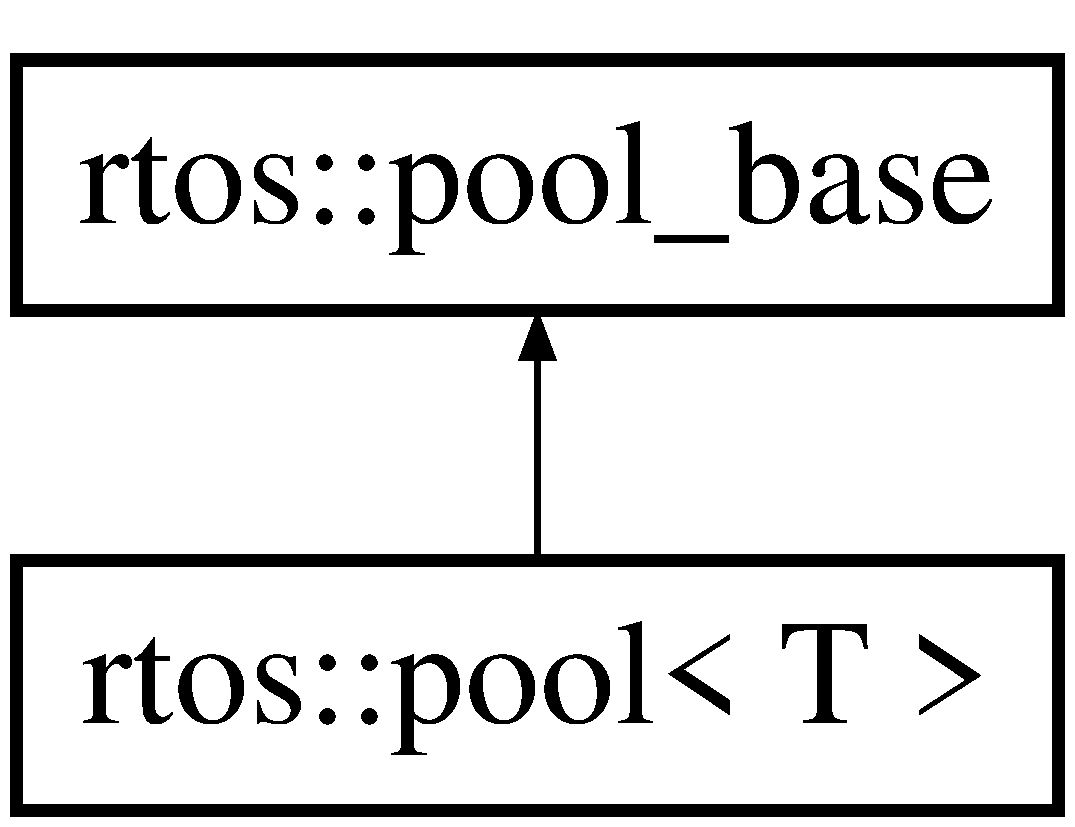
\includegraphics[height=2.000000cm]{classrtos_1_1pool}
\end{center}
\end{figure}
\subsection*{Public Member Functions}
\begin{DoxyCompactItemize}
\item 
\hyperlink{classrtos_1_1pool_a5112915f2ae720f6f49972bef2668a6d}{pool} (const char $\ast$name=\char`\"{}\char`\"{})
\begin{DoxyCompactList}\small\item\em construct a pool, specify its name (for debgging only) \end{DoxyCompactList}\item 
void \hyperlink{classrtos_1_1pool_a9a6f29c8b3daf17064e22ec4c4a47dfa}{write} (T item)
\begin{DoxyCompactList}\small\item\em atomic write operation on a pool \end{DoxyCompactList}\item 
T \hyperlink{classrtos_1_1pool_ad3e243cb97b89b891f3683dce82cafd8}{read} (void)
\begin{DoxyCompactList}\small\item\em atomic read operation on a pool \end{DoxyCompactList}\end{DoxyCompactItemize}
\subsection*{Additional Inherited Members}


\subsection{Detailed Description}
\subsubsection*{template$<$class T$>$\\*
class rtos\+::pool$<$ T $>$}

place to store and rectrieve data, no built-\/in synchronisation 

A (communication) pool is a template class that stores a single value. It supports the read and write operations, which are guaranteed to be atomic. (On a non-\/preemptive rtos every assignment is atomic, but the pool template is still usefull to make it explicit that data is transferred between tasks.) A pool is just a variable.

The example below demonstrates the use of a pool to maintain a seconds-\/since-\/startup counter. Note that the call rtos\+::runtime() returns the time elapsed since startup, so there is no need to maintain a seconds-\/since-\/startup this way yourself.


\begin{DoxyCode}
pool< unsigned int > seconds;

\textcolor{keywordtype}{void} show\_time( \textcolor{keywordtype}{void} )\{
   \textcolor{keywordtype}{unsigned} \textcolor{keywordtype}{int} n = seconds.read();
   std::cout << ( seconds / 60 ) % 60 << \textcolor{stringliteral}{":"} << seconds % 60;
\}

\textcolor{keyword}{class }seconds\_counter\_class : \textcolor{keyword}{public} periodic\_task \{
   seconds\_counter( \textcolor{keywordtype}{void} )\{
      periodic\_task::periodic\_task( \textcolor{stringliteral}{"sec-counter"}, 10, 1000 MS );
      seconds.write( 0 );
   \}
   \textcolor{keywordtype}{void} main( \textcolor{keywordtype}{void} )\{
      \textcolor{keywordflow}{for}( ; ; ) \{
         (void) wait(); \textcolor{comment}{// only one thing to wait for}
         seconds.write( seconds.read() + 1 );
      \}
   \}
\}

seconds\_counter\_class seconds\_counter;
\end{DoxyCode}
 

\subsection{Constructor \& Destructor Documentation}
\index{rtos\+::pool@{rtos\+::pool}!pool@{pool}}
\index{pool@{pool}!rtos\+::pool@{rtos\+::pool}}
\subsubsection[{\texorpdfstring{pool(const char $\ast$name="""")}{pool(const char *name="")}}]{\setlength{\rightskip}{0pt plus 5cm}template$<$class T $>$ {\bf rtos\+::pool}$<$ T $>$\+::{\bf pool} (
\begin{DoxyParamCaption}
\item[{const char $\ast$}]{name = {\ttfamily \char`\"{}\char`\"{}}}
\end{DoxyParamCaption}
)\hspace{0.3cm}{\ttfamily [inline]}}\hypertarget{classrtos_1_1pool_a5112915f2ae720f6f49972bef2668a6d}{}\label{classrtos_1_1pool_a5112915f2ae720f6f49972bef2668a6d}


construct a pool, specify its name (for debgging only) 

Use it to make (global) variables use for communication between tasks explicit.

The template argument T must be a class that has a non-\/arguments constructor and supports assignment. 

\subsection{Member Function Documentation}
\index{rtos\+::pool@{rtos\+::pool}!read@{read}}
\index{read@{read}!rtos\+::pool@{rtos\+::pool}}
\subsubsection[{\texorpdfstring{read(void)}{read(void)}}]{\setlength{\rightskip}{0pt plus 5cm}template$<$class T $>$ T {\bf rtos\+::pool}$<$ T $>$\+::read (
\begin{DoxyParamCaption}
\item[{void}]{}
\end{DoxyParamCaption}
)\hspace{0.3cm}{\ttfamily [inline]}}\hypertarget{classrtos_1_1pool_ad3e243cb97b89b891f3683dce82cafd8}{}\label{classrtos_1_1pool_ad3e243cb97b89b891f3683dce82cafd8}


atomic read operation on a pool 

A read opeartion returns the most recently written data.

In the context of co-\/operative multitasking a read of write operation on anything is always atomic, unless the implementation of that operating somehow invokes the rtos. But for clearness it is a good idea to implement such task-\/global data as pools. \index{rtos\+::pool@{rtos\+::pool}!write@{write}}
\index{write@{write}!rtos\+::pool@{rtos\+::pool}}
\subsubsection[{\texorpdfstring{write(\+T item)}{write(T item)}}]{\setlength{\rightskip}{0pt plus 5cm}template$<$class T $>$ void {\bf rtos\+::pool}$<$ T $>$\+::write (
\begin{DoxyParamCaption}
\item[{T}]{item}
\end{DoxyParamCaption}
)\hspace{0.3cm}{\ttfamily [inline]}}\hypertarget{classrtos_1_1pool_a9a6f29c8b3daf17064e22ec4c4a47dfa}{}\label{classrtos_1_1pool_a9a6f29c8b3daf17064e22ec4c4a47dfa}


atomic write operation on a pool 

A read opeartion returns the most recently written data.

In the context of co-\/operative multitasking a read of write operation on anything is always atomic, unless the implementation of that operating somehow invokes the rtos. But for clearness it is a good idea to implement such task-\/global data as pools. 

The documentation for this class was generated from the following file\+:\begin{DoxyCompactItemize}
\item 
rtos.\+hpp\end{DoxyCompactItemize}

\hypertarget{classrtos_1_1pool__base}{}\section{rtos\+:\+:pool\+\_\+base Class Reference}
\label{classrtos_1_1pool__base}\index{rtos\+::pool\+\_\+base@{rtos\+::pool\+\_\+base}}


rtos private implementation class  




{\ttfamily \#include $<$rtos.\+hpp$>$}

Inheritance diagram for rtos\+:\+:pool\+\_\+base\+:\begin{figure}[H]
\begin{center}
\leavevmode
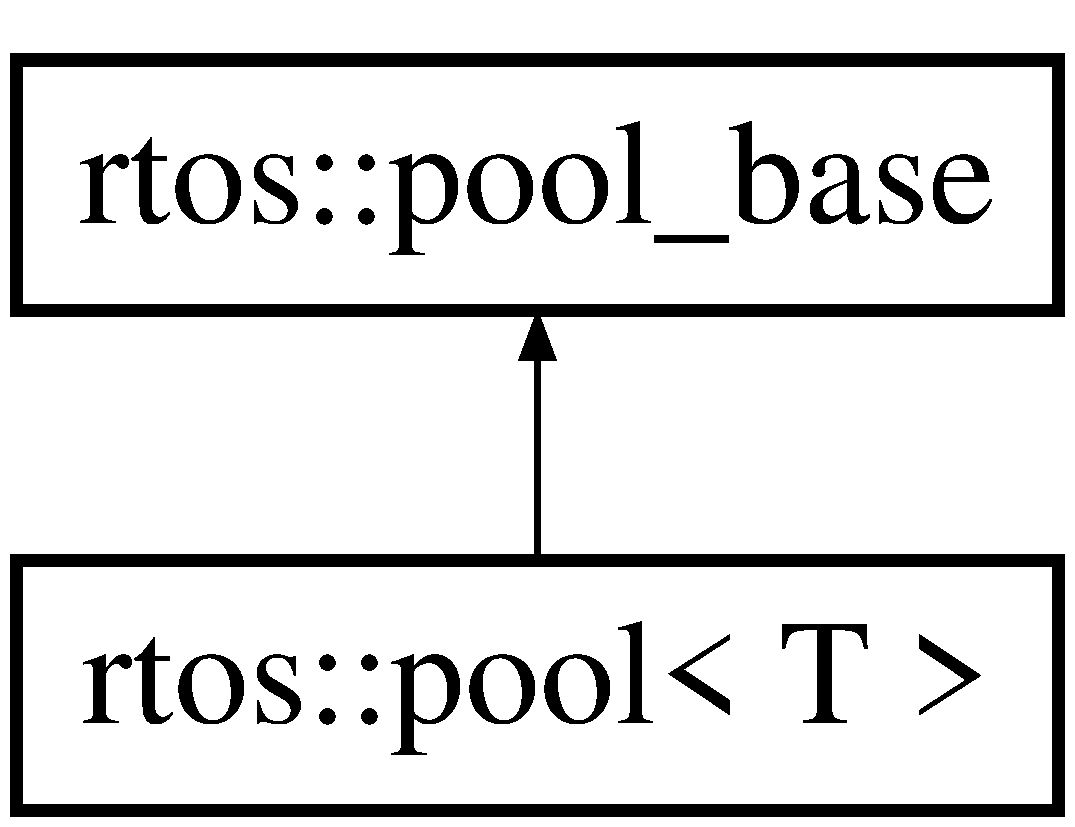
\includegraphics[height=2.000000cm]{classrtos_1_1pool__base}
\end{center}
\end{figure}
\subsection*{Public Member Functions}
\begin{DoxyCompactItemize}
\item 
{\bfseries pool\+\_\+base} (const char $\ast$name)\hypertarget{classrtos_1_1pool__base_a80e1aa93f3b8892060339f8ced055a1c}{}\label{classrtos_1_1pool__base_a80e1aa93f3b8892060339f8ced055a1c}

\item 
void {\bfseries print} (hwlib\+::ostream \&s, bool header=true) const \hypertarget{classrtos_1_1pool__base_ad4933e03799b48987874803a17065a05}{}\label{classrtos_1_1pool__base_ad4933e03799b48987874803a17065a05}

\end{DoxyCompactItemize}
\subsection*{Public Attributes}
\begin{DoxyCompactItemize}
\item 
unsigned int {\bfseries reads}\hypertarget{classrtos_1_1pool__base_af1d2c0ebc43cdf86eb369d8e181fc2c7}{}\label{classrtos_1_1pool__base_af1d2c0ebc43cdf86eb369d8e181fc2c7}

\item 
unsigned int {\bfseries writes}\hypertarget{classrtos_1_1pool__base_a85103a528d8dac5e40262cc39968a7f6}{}\label{classrtos_1_1pool__base_a85103a528d8dac5e40262cc39968a7f6}

\item 
\hyperlink{classrtos_1_1pool__base}{pool\+\_\+base} $\ast$ {\bfseries next\+\_\+pool}\hypertarget{classrtos_1_1pool__base_a123094ff55fa3f599059a6133168f7cc}{}\label{classrtos_1_1pool__base_a123094ff55fa3f599059a6133168f7cc}

\item 
const char $\ast$ {\bfseries pool\+\_\+name}\hypertarget{classrtos_1_1pool__base_aa546f6f4b86abc5878edaaaf4560ef70}{}\label{classrtos_1_1pool__base_aa546f6f4b86abc5878edaaaf4560ef70}

\end{DoxyCompactItemize}
\subsection*{Friends}
\begin{DoxyCompactItemize}
\item 
class {\bfseries rtos}\hypertarget{classrtos_1_1pool__base_a2a7bcfc34141352757ad672e3ecd099f}{}\label{classrtos_1_1pool__base_a2a7bcfc34141352757ad672e3ecd099f}

\end{DoxyCompactItemize}


\subsection{Detailed Description}
rtos private implementation class 

The documentation for this class was generated from the following files\+:\begin{DoxyCompactItemize}
\item 
rtos.\+hpp\item 
rtos.\+cpp\end{DoxyCompactItemize}

\hypertarget{classrtos}{}\section{rtos Class Reference}
\label{classrtos}\index{rtos@{rtos}}


static class, namespace-\/like container for R\+T\+OS declarations  




{\ttfamily \#include $<$rtos.\+hpp$>$}

\subsection*{Classes}
\begin{DoxyCompactItemize}
\item 
class \hyperlink{classrtos_1_1channel}{channel}
\begin{DoxyCompactList}\small\item\em waitable data queue \end{DoxyCompactList}\item 
class \hyperlink{classrtos_1_1channel__base}{channel\+\_\+base}
\begin{DoxyCompactList}\small\item\em rtos private implementation class \end{DoxyCompactList}\item 
class \hyperlink{classrtos_1_1clock}{clock}
\begin{DoxyCompactList}\small\item\em free-\/running clock, ticks at a fixed frequency \end{DoxyCompactList}\item 
class \hyperlink{classrtos_1_1event}{event}
\begin{DoxyCompactList}\small\item\em set of things that can happen, or a thing that has happened \end{DoxyCompactList}\item 
class \hyperlink{classrtos_1_1flag}{flag}
\begin{DoxyCompactList}\small\item\em basic synchronisation mechanism. \end{DoxyCompactList}\item 
class \hyperlink{classrtos_1_1mailbox}{mailbox}
\begin{DoxyCompactList}\small\item\em Synchronously handing over of a data item. \end{DoxyCompactList}\item 
class \hyperlink{classrtos_1_1mailbox__base}{mailbox\+\_\+base}
\begin{DoxyCompactList}\small\item\em rtos private implementation class \end{DoxyCompactList}\item 
class \hyperlink{classrtos_1_1mutex}{mutex}
\begin{DoxyCompactList}\small\item\em mutual execlusion semaphore \end{DoxyCompactList}\item 
class \hyperlink{classrtos_1_1pool}{pool}
\begin{DoxyCompactList}\small\item\em place to store and rectrieve data, no built-\/in synchronisation \end{DoxyCompactList}\item 
class \hyperlink{classrtos_1_1pool__base}{pool\+\_\+base}
\begin{DoxyCompactList}\small\item\em rtos private implementation class \end{DoxyCompactList}\item 
class \hyperlink{classrtos_1_1task}{task}
\item 
class \hyperlink{classrtos_1_1task__base}{task\+\_\+base}
\begin{DoxyCompactList}\small\item\em an independent thread of execution \end{DoxyCompactList}\item 
class \hyperlink{classrtos_1_1timer}{timer}
\begin{DoxyCompactList}\small\item\em one-\/short timer \end{DoxyCompactList}\item 
class \hyperlink{classrtos_1_1waitable}{waitable}
\begin{DoxyCompactList}\small\item\em abstract thing that a task can wait for \end{DoxyCompactList}\end{DoxyCompactItemize}
\subsection*{Static Public Member Functions}
\begin{DoxyCompactItemize}
\item 
static void \hyperlink{classrtos_a1b1490e971b7908f28f7af9cfb18e5aa}{run} (void)\hypertarget{classrtos_a1b1490e971b7908f28f7af9cfb18e5aa}{}\label{classrtos_a1b1490e971b7908f28f7af9cfb18e5aa}

\begin{DoxyCompactList}\small\item\em runs the scheduler \end{DoxyCompactList}\item 
static \hyperlink{classrtos_1_1task__base}{task\+\_\+base} $\ast$ \hyperlink{classrtos_aebecb7a849f7d692fea474aae864ccc2}{current\+\_\+task} (void)\hypertarget{classrtos_aebecb7a849f7d692fea474aae864ccc2}{}\label{classrtos_aebecb7a849f7d692fea474aae864ccc2}

\begin{DoxyCompactList}\small\item\em returns (a pointer to) the currently executing task \end{DoxyCompactList}\item 
static long long int \hyperlink{classrtos_a9f271842ab57becb8d51b248cb000ebb}{run\+\_\+time} (void)\hypertarget{classrtos_a9f271842ab57becb8d51b248cb000ebb}{}\label{classrtos_a9f271842ab57becb8d51b248cb000ebb}

\begin{DoxyCompactList}\small\item\em get elapsed time in micro seconds since OS startup \end{DoxyCompactList}\item 
static void \hyperlink{classrtos_a89f20236423a5523ee6630613bf3d294}{print} (hwlib\+::ostream \&stream)\hypertarget{classrtos_a89f20236423a5523ee6630613bf3d294}{}\label{classrtos_a89f20236423a5523ee6630613bf3d294}

\begin{DoxyCompactList}\small\item\em prints statistics about the R\+T\+OS to the stream. \end{DoxyCompactList}\item 
static void \hyperlink{classrtos_ac72c2b921526d55e1c7557acefdec823}{statistics\+\_\+clear} (void)
\begin{DoxyCompactList}\small\item\em clears the statistics. \end{DoxyCompactList}\item 
static void \hyperlink{classrtos_a678def9714d83696d5b174e45481139a}{display\+\_\+statistics} (void)\hypertarget{classrtos_a678def9714d83696d5b174e45481139a}{}\label{classrtos_a678def9714d83696d5b174e45481139a}

\begin{DoxyCompactList}\small\item\em print the statistics collect for the used R\+T\+OS objects \end{DoxyCompactList}\end{DoxyCompactItemize}
\subsection*{Static Public Attributes}
\begin{DoxyCompactItemize}
\item 
static const long long int {\bfseries us} = 84\hypertarget{classrtos_a69a2d0d58bbc0f4a40a3f33c367139b5}{}\label{classrtos_a69a2d0d58bbc0f4a40a3f33c367139b5}

\item 
static const long long int {\bfseries ms} = ( 1000 $\ast$ us )\hypertarget{classrtos_a36eea8062f297b913190576fd25e41a5}{}\label{classrtos_a36eea8062f297b913190576fd25e41a5}

\item 
static const long long int {\bfseries s} = ( 1000 $\ast$ ms )\hypertarget{classrtos_a0519ae662d39eb04dfd7c87593ee124c}{}\label{classrtos_a0519ae662d39eb04dfd7c87593ee124c}

\end{DoxyCompactItemize}
\subsection*{Friends}
\begin{DoxyCompactItemize}
\item 
void {\bfseries hwlib\+::wait\+\_\+us} (int\+\_\+fast32\+\_\+t n)\hypertarget{classrtos_a93f92abd9f492627db6ff42b0cfd256b}{}\label{classrtos_a93f92abd9f492627db6ff42b0cfd256b}

\end{DoxyCompactItemize}


\subsection{Detailed Description}
static class, namespace-\/like container for R\+T\+OS declarations 

The R\+T\+OS is a static class, instantiation is not needed. After creating the tasks, call R\+T\+O\+S\+::run() to start the scheduling of the tasks. R\+T\+O\+S\+::run() will never return. 

\subsection{Member Function Documentation}
\index{rtos@{rtos}!statistics\+\_\+clear@{statistics\+\_\+clear}}
\index{statistics\+\_\+clear@{statistics\+\_\+clear}!rtos@{rtos}}
\subsubsection[{\texorpdfstring{statistics\+\_\+clear(void)}{statistics_clear(void)}}]{\setlength{\rightskip}{0pt plus 5cm}static void rtos\+::statistics\+\_\+clear (
\begin{DoxyParamCaption}
\item[{void}]{}
\end{DoxyParamCaption}
)\hspace{0.3cm}{\ttfamily [inline]}, {\ttfamily [static]}}\hypertarget{classrtos_ac72c2b921526d55e1c7557acefdec823}{}\label{classrtos_ac72c2b921526d55e1c7557acefdec823}


clears the statistics. 

The actual clearing will be done later, inside \hyperlink{classrtos_a1b1490e971b7908f28f7af9cfb18e5aa}{run()}, when the current task has given up the processor. 

The documentation for this class was generated from the following files\+:\begin{DoxyCompactItemize}
\item 
rtos.\+hpp\item 
rtos.\+cpp\end{DoxyCompactItemize}

\hypertarget{classrtos_1_1task}{}\section{rtos\+:\+:task$<$ N $>$ Class Template Reference}
\label{classrtos_1_1task}\index{rtos\+::task$<$ N $>$@{rtos\+::task$<$ N $>$}}
Inheritance diagram for rtos\+:\+:task$<$ N $>$\+:\begin{figure}[H]
\begin{center}
\leavevmode
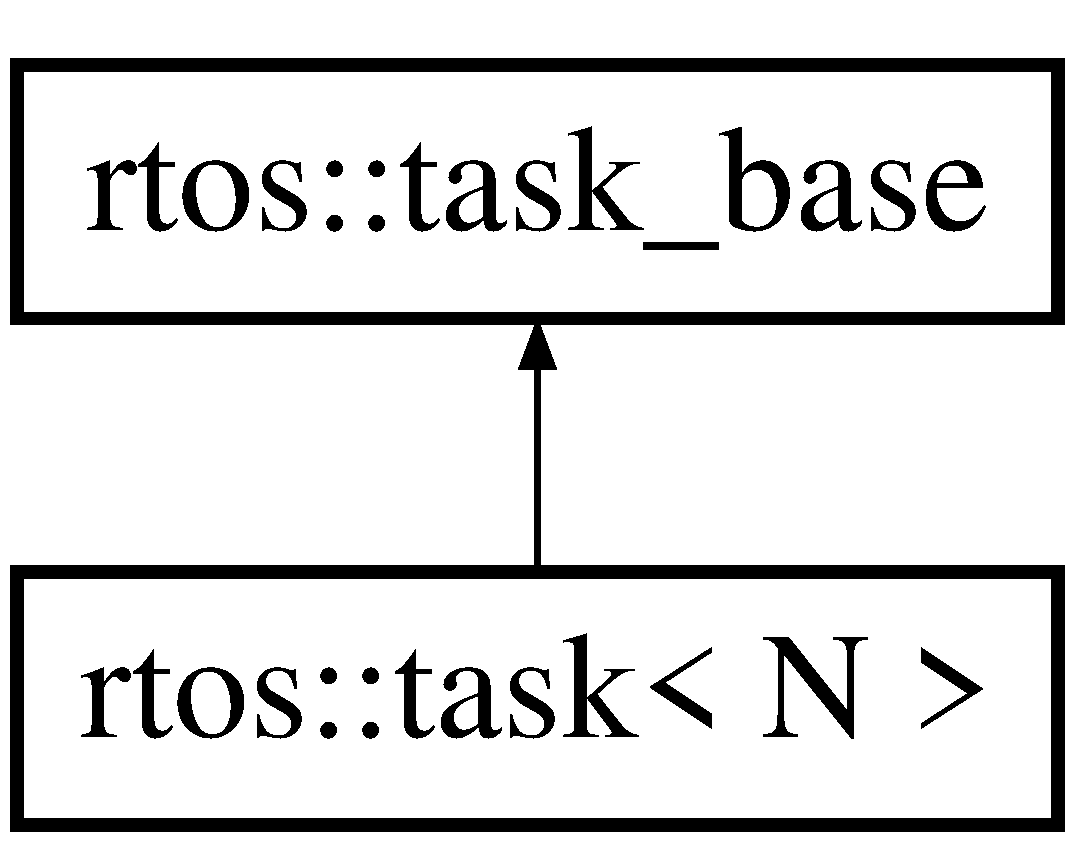
\includegraphics[height=2.000000cm]{classrtos_1_1task}
\end{center}
\end{figure}
\subsection*{Public Member Functions}
\begin{DoxyCompactItemize}
\item 
{\bfseries task} (unsigned int \hyperlink{classrtos_1_1task__base_aca1f728cef4c3e70e1ce08b6e313b586}{priority}=R\+T\+O\+S\+\_\+\+M\+I\+N\+\_\+\+P\+R\+I\+O\+R\+I\+TY, const char $\ast$tname=\char`\"{}\char`\"{})\hypertarget{classrtos_1_1task_a36f4e4a5aa5bfbcf35df75858d4d5abd}{}\label{classrtos_1_1task_a36f4e4a5aa5bfbcf35df75858d4d5abd}

\item 
{\bfseries task} (const char $\ast$tname)\hypertarget{classrtos_1_1task_a524617b96daa37e19fe438ec4eb866f0}{}\label{classrtos_1_1task_a524617b96daa37e19fe438ec4eb866f0}

\end{DoxyCompactItemize}


The documentation for this class was generated from the following file\+:\begin{DoxyCompactItemize}
\item 
rtos.\+hpp\end{DoxyCompactItemize}

\hypertarget{classrtos_1_1task__base}{}\section{rtos\+:\+:task\+\_\+base Class Reference}
\label{classrtos_1_1task__base}\index{rtos\+::task\+\_\+base@{rtos\+::task\+\_\+base}}


an independent thread of execution  




{\ttfamily \#include $<$rtos.\+hpp$>$}

Inheritance diagram for rtos\+:\+:task\+\_\+base\+:\begin{figure}[H]
\begin{center}
\leavevmode
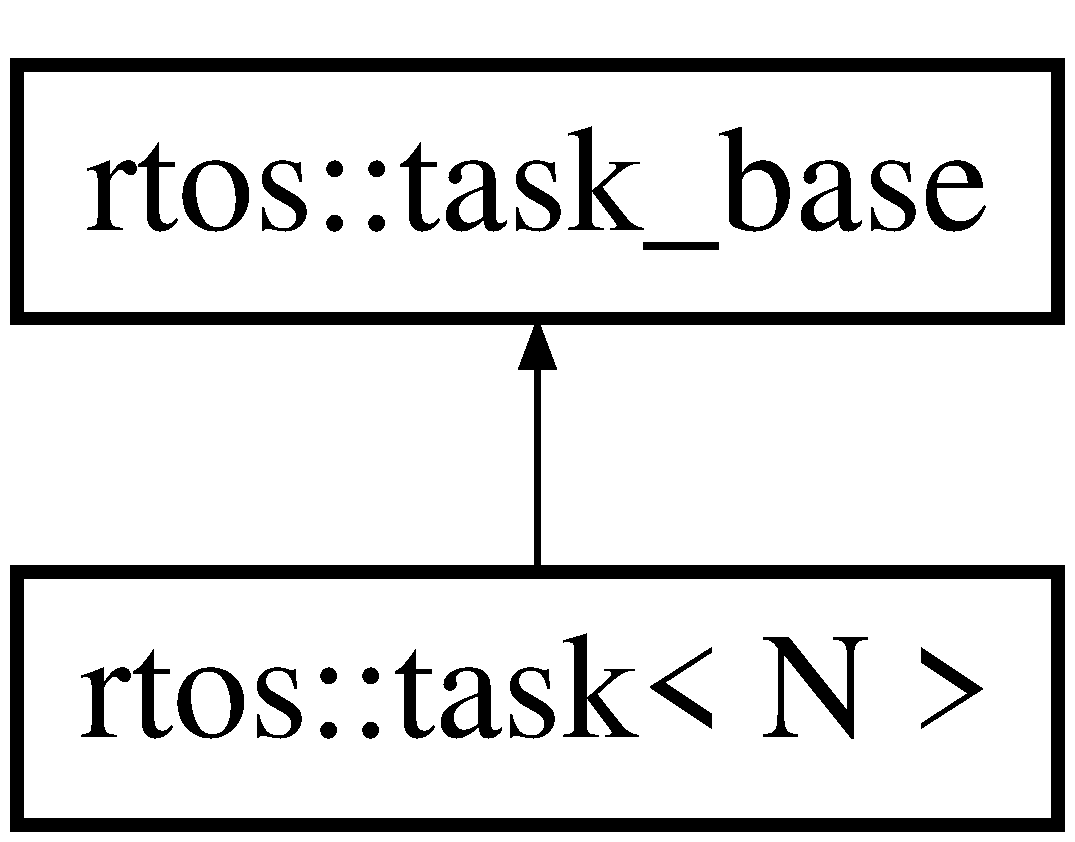
\includegraphics[height=2.000000cm]{classrtos_1_1task__base}
\end{center}
\end{figure}
\subsection*{Public Member Functions}
\begin{DoxyCompactItemize}
\item 
virtual void \hyperlink{classrtos_1_1task__base_a35016dfecdd20ce4786ef7a16154976a}{main} (void)=0
\begin{DoxyCompactList}\small\item\em task body, must be provided by a derived class \end{DoxyCompactList}\item 
\hyperlink{classrtos_1_1task__base_aa7a9351a480725a93f1c2f99451e28e2}{task\+\_\+base} (\hyperlink{classcoroutine}{coroutine}$<$$>$ \&cor, unsigned int \hyperlink{classrtos_1_1task__base_aca1f728cef4c3e70e1ce08b6e313b586}{priority}=R\+T\+O\+S\+\_\+\+M\+I\+N\+\_\+\+P\+R\+I\+O\+R\+I\+TY, const char $\ast$tname=\char`\"{}\char`\"{})
\begin{DoxyCompactList}\small\item\em constructor, specify priority, name and stack size \end{DoxyCompactList}\item 
\hyperlink{classrtos_1_1task__base_a8df882df03cd39af4f21609ba1e002e4}{$\sim$task\+\_\+base} ()\hypertarget{classrtos_1_1task__base_a8df882df03cd39af4f21609ba1e002e4}{}\label{classrtos_1_1task__base_a8df882df03cd39af4f21609ba1e002e4}

\begin{DoxyCompactList}\small\item\em throws an error, beacuse tasks should never be destroyed \end{DoxyCompactList}\item 
virtual void \hyperlink{classrtos_1_1task__base_a2e5c57f7993ffa43c91348277ec2478c}{suspend} (void)
\begin{DoxyCompactList}\small\item\em suspend a task (prevent execution until a resume) \end{DoxyCompactList}\item 
virtual void \hyperlink{classrtos_1_1task__base_a4e9601dcea7c1d392b05ebd4f921de04}{resume} (void)
\begin{DoxyCompactList}\small\item\em continue a suspended task \end{DoxyCompactList}\item 
void \hyperlink{classrtos_1_1task__base_a0b397b5bbdbfdeea5be6c6b505b5e266}{release} (void)
\begin{DoxyCompactList}\small\item\em release the C\+PU to the scheduler \end{DoxyCompactList}\item 
void \hyperlink{classrtos_1_1task__base_a1110fdfe776e7f256eb809216e97c836}{sleep} (unsigned int time)
\begin{DoxyCompactList}\small\item\em wait for some time \end{DoxyCompactList}\item 
unsigned int \hyperlink{classrtos_1_1task__base_aca1f728cef4c3e70e1ce08b6e313b586}{priority} (void) const \hypertarget{classrtos_1_1task__base_aca1f728cef4c3e70e1ce08b6e313b586}{}\label{classrtos_1_1task__base_aca1f728cef4c3e70e1ce08b6e313b586}

\begin{DoxyCompactList}\small\item\em report the task priority \end{DoxyCompactList}\item 
const char $\ast$ \hyperlink{classrtos_1_1task__base_ad6469d5653e3021769e4fa89c20920bf}{name} (void) const \hypertarget{classrtos_1_1task__base_ad6469d5653e3021769e4fa89c20920bf}{}\label{classrtos_1_1task__base_ad6469d5653e3021769e4fa89c20920bf}

\begin{DoxyCompactList}\small\item\em report the task name \end{DoxyCompactList}\item 
bool \hyperlink{classrtos_1_1task__base_ae62a76e0a7fd1548077eb26481b52dee}{is\+\_\+suspended} (void) const \hypertarget{classrtos_1_1task__base_ae62a76e0a7fd1548077eb26481b52dee}{}\label{classrtos_1_1task__base_ae62a76e0a7fd1548077eb26481b52dee}

\begin{DoxyCompactList}\small\item\em report whether the task is currently suspended \end{DoxyCompactList}\item 
bool \hyperlink{classrtos_1_1task__base_a239db2650c0258d52c73bfa386455476}{is\+\_\+blocked} (void) const \hypertarget{classrtos_1_1task__base_a239db2650c0258d52c73bfa386455476}{}\label{classrtos_1_1task__base_a239db2650c0258d52c73bfa386455476}

\begin{DoxyCompactList}\small\item\em report whether the task is currently blocked \end{DoxyCompactList}\item 
bool \hyperlink{classrtos_1_1task__base_a2da0d689fd9d9546483a83e8787d0ad8}{is\+\_\+ready} (void) const \hypertarget{classrtos_1_1task__base_a2da0d689fd9d9546483a83e8787d0ad8}{}\label{classrtos_1_1task__base_a2da0d689fd9d9546483a83e8787d0ad8}

\begin{DoxyCompactList}\small\item\em report whether the task is currently ready for execution \end{DoxyCompactList}\item 
void \hyperlink{classrtos_1_1task__base_a0b79c3c2b76ce32284638467cec95c65}{print} (hwlib\+::ostream \&stream, bool header=true) const \hypertarget{classrtos_1_1task__base_a0b79c3c2b76ce32284638467cec95c65}{}\label{classrtos_1_1task__base_a0b79c3c2b76ce32284638467cec95c65}

\begin{DoxyCompactList}\small\item\em print task statistics \end{DoxyCompactList}\item 
\hyperlink{classrtos_1_1event}{event} \hyperlink{classrtos_1_1task__base_a2590ba76480cecaff66282516fbeb1bb}{wait} (void)
\begin{DoxyCompactList}\small\item\em wait for all waitables created for this task \end{DoxyCompactList}\item 
\hyperlink{classrtos_1_1event}{event} \hyperlink{classrtos_1_1task__base_a52035722f108687680966b87dd60bfe1}{wait} (const \hyperlink{classrtos_1_1waitable}{waitable} \&w)
\begin{DoxyCompactList}\small\item\em wait for a single waitable \end{DoxyCompactList}\item 
\hyperlink{classrtos_1_1event}{event} \hyperlink{classrtos_1_1task__base_a6acecfe733161a6258d39ed7a49275d0}{wait} (const \hyperlink{classrtos_1_1event}{event} \&\hyperlink{classrtos_1_1task__base_a1b3cb75ba2ef779cffc76b6076ecac39}{set})
\begin{DoxyCompactList}\small\item\em wait for a set of waitables \end{DoxyCompactList}\item 
void \hyperlink{classrtos_1_1task__base_a1b3cb75ba2ef779cffc76b6076ecac39}{set} (\hyperlink{classrtos_1_1flag}{flag} \&f)\hypertarget{classrtos_1_1task__base_a1b3cb75ba2ef779cffc76b6076ecac39}{}\label{classrtos_1_1task__base_a1b3cb75ba2ef779cffc76b6076ecac39}

\begin{DoxyCompactList}\small\item\em set a flag \end{DoxyCompactList}\item 
void \hyperlink{classrtos_1_1task__base_a31d2bfe971b2c526125d5a670d8465f4}{ignore\+\_\+activation\+\_\+time} (void)
\begin{DoxyCompactList}\small\item\em ignore this activation for the statistics \end{DoxyCompactList}\end{DoxyCompactItemize}
\subsection*{Friends}
\begin{DoxyCompactItemize}
\item 
class {\bfseries periodic\+\_\+task}\hypertarget{classrtos_1_1task__base_a01d2f5a71b8cd797b5f01fb6940ea353}{}\label{classrtos_1_1task__base_a01d2f5a71b8cd797b5f01fb6940ea353}

\item 
class {\bfseries waitable\+\_\+set}\hypertarget{classrtos_1_1task__base_a0ee29d8961a0b67cea2c3fa76da116da}{}\label{classrtos_1_1task__base_a0ee29d8961a0b67cea2c3fa76da116da}

\item 
class {\bfseries flag}\hypertarget{classrtos_1_1task__base_a2d8be07618a92a592c4905e969f9927f}{}\label{classrtos_1_1task__base_a2d8be07618a92a592c4905e969f9927f}

\item 
class {\bfseries rtos}\hypertarget{classrtos_1_1task__base_a2a7bcfc34141352757ad672e3ecd099f}{}\label{classrtos_1_1task__base_a2a7bcfc34141352757ad672e3ecd099f}

\item 
void {\bfseries task\+\_\+trampoline} ()\hypertarget{classrtos_1_1task__base_a376fdffc11fe9fb4f531835b94320825}{}\label{classrtos_1_1task__base_a376fdffc11fe9fb4f531835b94320825}

\end{DoxyCompactItemize}


\subsection{Detailed Description}
an independent thread of execution 

A task is an independent thread of execution, using its own stack. Tasks share the single C\+PU, so only one task can be running at any time. The rtos determines which task is running. A task has two bi-\/value states that determine whether the task is runnable\+: the suspended/resumed flag and the waiting/non-\/waiting flag. A task is runnable only when it is both resumed, and non-\/waiting. When a task is created it is resumed and non-\/waiting. All tasks (and the rtos code) run in the same memory space, without protection from each other. So a \textquotesingle{}wild pointer\textquotesingle{} in one task can destroy data in another task, or even in the rtos.

Each task is created with a fixed priority, which can be any unsigned integer value below R\+T\+O\+S\+\_\+\+M\+I\+N\+\_\+\+P\+R\+I\+O\+R\+I\+TY (= 1000). After creation the priority can not be changed. The value 0 indicates the highest task priority, a higher number indicates a lower priority. Each task must have a unique priority, it is an error to create a task with same priority as an existing task. You can omit the priority, in which case the R\+T\+OS will select an unused priority starting at R\+T\+O\+S\+\_\+\+M\+I\+N\+\_\+\+P\+R\+I\+O\+R\+I\+TY (in other words, it will choose a low priority for your task).

Each task has its own stack. You can specify the size of the stack at task creation. If you omit the stack size, R\+T\+O\+S\+\_\+\+D\+E\+F\+A\+U\+L\+T\+\_\+\+S\+T\+A\+C\+K\+\_\+\+S\+I\+ZE will be used (default\+: 8 Kb). This will be enough for most tasks, if you take care not to allocate big things on the stack, and avoid very deep nesting (watch out for recursion!).

A task is created by instatiating a class that derives from \hyperlink{classrtos_1_1task}{rtos\+::task} and supplies a \hyperlink{classrtos_1_1task__base_a35016dfecdd20ce4786ef7a16154976a}{main()}. This \hyperlink{classrtos_1_1task__base_a35016dfecdd20ce4786ef7a16154976a}{main()} should never return. The fragment below shows how you can do this. The task name is used for statistics and debugging. As shown for the name, it might be wise to get the task parameters as arguments to the constructor of your task.


\begin{DoxyCode}
\textcolor{keyword}{class }my\_task\_class : \textcolor{keyword}{public} \hyperlink{classrtos_1_1task}{rtos::task} \{
\textcolor{keyword}{public}:
   my\_task\_class( \textcolor{keyword}{const} \textcolor{keywordtype}{char} * \hyperlink{classrtos_1_1task__base_ad6469d5653e3021769e4fa89c20920bf}{name} ):
      task(
         name,  \textcolor{comment}{// name of the task}
         10,    \textcolor{comment}{// task priority}
         16384  \textcolor{comment}{// task stack size}
      )\{\}
\textcolor{keyword}{private}:
   \textcolor{keywordtype}{void} \hyperlink{classrtos_1_1task__base_a35016dfecdd20ce4786ef7a16154976a}{main}( \textcolor{keywordtype}{void} )\{
      \textcolor{comment}{// put the code of your task here}
   \}
\};
my\_task\_class my\_task( \textcolor{stringliteral}{"my first task"} );
my\_task\_class my\_task( \textcolor{stringliteral}{"my second task"} );
\end{DoxyCode}


The example below is a complete program that shows the standard part (initialization, and a main that calls \hyperlink{classrtos_a1b1490e971b7908f28f7af9cfb18e5aa}{rtos\+::run()}), a function for writing to an individual L\+ED, a task class that blinks a L\+ED, and two instatiations of this class. Note that the \hyperlink{classrtos_1_1task__base_a1110fdfe776e7f256eb809216e97c836}{sleep()} call is used instead of mkt\+\_\+wait\+\_\+ms or mkt\+\_\+wait\+\_\+us. Sleep() causes other tasks to run while this task is waiting, whereas the mkt\+\_\+wait\+\_\+$\ast$ calls would use monopolize the C\+PU to do a busy wait.

Subsequent examples will not show the standard initialization (the part up to the comment line).


\begin{DoxyCode}
\textcolor{preprocessor}{#include "rtos.h"}

\textcolor{keywordtype}{int} \hyperlink{classrtos_1_1task__base_a35016dfecdd20ce4786ef7a16154976a}{main}( \textcolor{keywordtype}{void} ) \{
   \hyperlink{classrtos_a1b1490e971b7908f28f7af9cfb18e5aa}{rtos::run}();
   \textcolor{keywordflow}{return} 0;
\}

\textcolor{comment}{// end of standard part}

\textcolor{keyword}{class }blinker : \textcolor{keyword}{public} \hyperlink{classrtos_1_1task}{rtos::task} \{
\textcolor{keyword}{public}:
   blinker( \textcolor{keywordtype}{int} LED, \textcolor{keywordtype}{int} period ):
      LED( LED ), period( period )\{\}
\textcolor{keyword}{private}:
   \textcolor{keywordtype}{int} LED, period;
   \textcolor{keywordtype}{void} \hyperlink{classrtos_1_1task__base_a35016dfecdd20ce4786ef7a16154976a}{main}( \textcolor{keywordtype}{void} )\{
      \textcolor{keywordflow}{for}( ; ; ) \{
         led\_set( LED, 1 );
         \hyperlink{classrtos_1_1task__base_a1110fdfe776e7f256eb809216e97c836}{sleep}( period / 2 );
         led\_set( LED, 0 );
         \hyperlink{classrtos_1_1task__base_a1110fdfe776e7f256eb809216e97c836}{sleep}( period / 2 );
      \}
   \}
\};

blinker led0( 0, 1000 MS );
blinker led1( 1,  300 MS );
\end{DoxyCode}


A task can be suspended and resumed by the \hyperlink{classrtos_1_1task__base_a2e5c57f7993ffa43c91348277ec2478c}{task\+::suspend()} and \hyperlink{classrtos_1_1task__base_a4e9601dcea7c1d392b05ebd4f921de04}{task\+::resume()} calls. The suspend/resume state does not count the number of suspends and resumes\+: a suspend call on an already suspended task (or a resume on an already resumed task) has no effect. Suspend and resume are intended for use by the application code\+: the rtos will never suspend or resume a task. (The rtos uses the waiting/non-\/waiting state, which can not be changed directly by the application.)

The example below shows one task that beeps the speaker at 1 k\+Hz, while the other taks suspends and resumes the first task to make it beep 5 times, after which it suspends itself, which ends all activity. (This will trigger the rtos deadlock detection, because a normal embedded application should never terminate.)


\begin{DoxyCode}
\textcolor{keyword}{class }beeper : \textcolor{keyword}{public} \hyperlink{classrtos_1_1task}{rtos::task} \{
\textcolor{keyword}{public}:
   \textcolor{keywordtype}{unsigned} \textcolor{keywordtype}{int} speaker;
   beeper( \textcolor{keywordtype}{unsigned} \textcolor{keywordtype}{int} speaker ): speaker( speaker )\{\}
   \textcolor{keywordtype}{void} \hyperlink{classrtos_1_1task__base_a35016dfecdd20ce4786ef7a16154976a}{main}( \textcolor{keywordtype}{void} )\{
      mkt\_pin\_configure( speaker, mkt\_output);
      \textcolor{keywordflow}{for}( ; ; ) \{
         mkt\_pin\_write( speaker, 1  );
         \hyperlink{classrtos_1_1task__base_a1110fdfe776e7f256eb809216e97c836}{sleep}( 500 US );
         mkt\_pin\_write( speaker, 0  );
         \hyperlink{classrtos_1_1task__base_a1110fdfe776e7f256eb809216e97c836}{sleep}( 500 US );
      \}
   \}
\};
beeper speaker( 10 );

\textcolor{keyword}{class }suspender : \textcolor{keyword}{public} \hyperlink{classrtos_1_1task}{rtos::task} \{
   \textcolor{keywordtype}{void} \hyperlink{classrtos_1_1task__base_a35016dfecdd20ce4786ef7a16154976a}{main}( \textcolor{keywordtype}{void} )\{
      \textcolor{keywordflow}{for}( \textcolor{keywordtype}{int} i = 0; i < 5 ; i++ ) \{
         speaker.resume();
         \hyperlink{classrtos_1_1task__base_a1110fdfe776e7f256eb809216e97c836}{sleep}( 500 MS );
         speaker.suspend();
         \hyperlink{classrtos_1_1task__base_a1110fdfe776e7f256eb809216e97c836}{sleep}( 1 S );
      \}
      \hyperlink{classrtos_1_1task__base_a2e5c57f7993ffa43c91348277ec2478c}{suspend}();
   \}
\};
suspender task2;
\end{DoxyCode}
 

\subsection{Constructor \& Destructor Documentation}
\index{rtos\+::task\+\_\+base@{rtos\+::task\+\_\+base}!task\+\_\+base@{task\+\_\+base}}
\index{task\+\_\+base@{task\+\_\+base}!rtos\+::task\+\_\+base@{rtos\+::task\+\_\+base}}
\subsubsection[{\texorpdfstring{task\+\_\+base(coroutine$<$$>$ \&cor, unsigned int priority=\+R\+T\+O\+S\+\_\+\+M\+I\+N\+\_\+\+P\+R\+I\+O\+R\+I\+T\+Y, const char $\ast$tname="""")}{task_base(coroutine<> &cor, unsigned int priority=RTOS_MIN_PRIORITY, const char *tname="")}}]{\setlength{\rightskip}{0pt plus 5cm}rtos\+::task\+\_\+base\+::task\+\_\+base (
\begin{DoxyParamCaption}
\item[{{\bf coroutine}$<$$>$ \&}]{cor, }
\item[{unsigned int}]{priority = {\ttfamily RTOS\+\_\+MIN\+\_\+PRIORITY}, }
\item[{const char $\ast$}]{tname = {\ttfamily \char`\"{}\char`\"{}}}
\end{DoxyParamCaption}
)}\hypertarget{classrtos_1_1task__base_aa7a9351a480725a93f1c2f99451e28e2}{}\label{classrtos_1_1task__base_aa7a9351a480725a93f1c2f99451e28e2}


constructor, specify priority, name and stack size 

Priorities are reasonably-\/valued (below R\+T\+O\+S\+\_\+\+M\+I\+N\+\_\+\+P\+R\+I\+O\+R\+I\+TY) unsigned integers. 0 is te highest priority. Priorities must be unqiue. The default causes the constructor to choose a free priority starting at R\+T\+O\+S\+\_\+\+M\+I\+N\+\_\+\+P\+R\+I\+O\+R\+I\+TY (default\+: 1000).

The name is used for debugging and statistics.

A stack of stack\+\_\+size bytes is allocated for the task. The default is 4 kB. 

\subsection{Member Function Documentation}
\index{rtos\+::task\+\_\+base@{rtos\+::task\+\_\+base}!ignore\+\_\+activation\+\_\+time@{ignore\+\_\+activation\+\_\+time}}
\index{ignore\+\_\+activation\+\_\+time@{ignore\+\_\+activation\+\_\+time}!rtos\+::task\+\_\+base@{rtos\+::task\+\_\+base}}
\subsubsection[{\texorpdfstring{ignore\+\_\+activation\+\_\+time(void)}{ignore_activation_time(void)}}]{\setlength{\rightskip}{0pt plus 5cm}void rtos\+::task\+\_\+base\+::ignore\+\_\+activation\+\_\+time (
\begin{DoxyParamCaption}
\item[{void}]{}
\end{DoxyParamCaption}
)\hspace{0.3cm}{\ttfamily [inline]}}\hypertarget{classrtos_1_1task__base_a31d2bfe971b2c526125d5a670d8465f4}{}\label{classrtos_1_1task__base_a31d2bfe971b2c526125d5a670d8465f4}


ignore this activation for the statistics 

Calling this function makes the rtos statistics ignore the current task activation as far as statistics is concerned. You can use this to avoid pullution of your task statistics with the timing effects of debug logging. But make sure you don\textquotesingle{}t use it in the \textquotesingle{}normal\textquotesingle{} execution paths, because that would make the statistics lie to you. \index{rtos\+::task\+\_\+base@{rtos\+::task\+\_\+base}!main@{main}}
\index{main@{main}!rtos\+::task\+\_\+base@{rtos\+::task\+\_\+base}}
\subsubsection[{\texorpdfstring{main(void)=0}{main(void)=0}}]{\setlength{\rightskip}{0pt plus 5cm}virtual void rtos\+::task\+\_\+base\+::main (
\begin{DoxyParamCaption}
\item[{void}]{}
\end{DoxyParamCaption}
)\hspace{0.3cm}{\ttfamily [pure virtual]}}\hypertarget{classrtos_1_1task__base_a35016dfecdd20ce4786ef7a16154976a}{}\label{classrtos_1_1task__base_a35016dfecdd20ce4786ef7a16154976a}


task body, must be provided by a derived class 

A task is created by inheriting from task and providing a \hyperlink{classrtos_1_1task__base_a35016dfecdd20ce4786ef7a16154976a}{main()} function. Initialisation of the task, including creating its waitables, should be done in the constructor. Don\textquotesingle{}t forget to call the constructor of the task class!

The \hyperlink{classrtos_1_1task__base_a35016dfecdd20ce4786ef7a16154976a}{main()} is the body of the task. It should never terminate.

Each task has a unique priority (an unsigned integer). A lower value indicates a higher priority. The rtos scheduler will always run the task with the higest-\/priority runnable (neither blocked nor suspended) task. A task runs until it changes this \textquotesingle{}situation\textquotesingle{} by using an rtos call that changes its own state to not runnable, or the state of a higher priority task to runnable.

Timers are served only when the rtos is activated by calling any of its state-\/changing interfaces. Hence the longest run time between such calls determines the granularity (time wise responsiveness) of the application. Within a time consuming computation a task can call \hyperlink{classrtos_1_1task__base_a0b397b5bbdbfdeea5be6c6b505b5e266}{release()} to have the rtos serve the timers. \index{rtos\+::task\+\_\+base@{rtos\+::task\+\_\+base}!release@{release}}
\index{release@{release}!rtos\+::task\+\_\+base@{rtos\+::task\+\_\+base}}
\subsubsection[{\texorpdfstring{release(void)}{release(void)}}]{\setlength{\rightskip}{0pt plus 5cm}void rtos\+::task\+\_\+base\+::release (
\begin{DoxyParamCaption}
\item[{void}]{}
\end{DoxyParamCaption}
)}\hypertarget{classrtos_1_1task__base_a0b397b5bbdbfdeea5be6c6b505b5e266}{}\label{classrtos_1_1task__base_a0b397b5bbdbfdeea5be6c6b505b5e266}


release the C\+PU to the scheduler 

Sevices timers and releases the C\+PU to a higher priority task if is ready. \index{rtos\+::task\+\_\+base@{rtos\+::task\+\_\+base}!resume@{resume}}
\index{resume@{resume}!rtos\+::task\+\_\+base@{rtos\+::task\+\_\+base}}
\subsubsection[{\texorpdfstring{resume(void)}{resume(void)}}]{\setlength{\rightskip}{0pt plus 5cm}void rtos\+::task\+\_\+base\+::resume (
\begin{DoxyParamCaption}
\item[{void}]{}
\end{DoxyParamCaption}
)\hspace{0.3cm}{\ttfamily [virtual]}}\hypertarget{classrtos_1_1task__base_a4e9601dcea7c1d392b05ebd4f921de04}{}\label{classrtos_1_1task__base_a4e9601dcea7c1d392b05ebd4f921de04}


continue a suspended task 

Has no effect when the task is not suspended.

Can be extended by an application task to suit its needs. \index{rtos\+::task\+\_\+base@{rtos\+::task\+\_\+base}!sleep@{sleep}}
\index{sleep@{sleep}!rtos\+::task\+\_\+base@{rtos\+::task\+\_\+base}}
\subsubsection[{\texorpdfstring{sleep(unsigned int time)}{sleep(unsigned int time)}}]{\setlength{\rightskip}{0pt plus 5cm}void rtos\+::task\+\_\+base\+::sleep (
\begin{DoxyParamCaption}
\item[{unsigned int}]{time}
\end{DoxyParamCaption}
)}\hypertarget{classrtos_1_1task__base_a1110fdfe776e7f256eb809216e97c836}{}\label{classrtos_1_1task__base_a1110fdfe776e7f256eb809216e97c836}


wait for some time 

Sleeps the task (prevents execution) for the indicated time. \index{rtos\+::task\+\_\+base@{rtos\+::task\+\_\+base}!suspend@{suspend}}
\index{suspend@{suspend}!rtos\+::task\+\_\+base@{rtos\+::task\+\_\+base}}
\subsubsection[{\texorpdfstring{suspend(void)}{suspend(void)}}]{\setlength{\rightskip}{0pt plus 5cm}void rtos\+::task\+\_\+base\+::suspend (
\begin{DoxyParamCaption}
\item[{void}]{}
\end{DoxyParamCaption}
)\hspace{0.3cm}{\ttfamily [virtual]}}\hypertarget{classrtos_1_1task__base_a2e5c57f7993ffa43c91348277ec2478c}{}\label{classrtos_1_1task__base_a2e5c57f7993ffa43c91348277ec2478c}


suspend a task (prevent execution until a resume) 

Suspends the task (prevents execution). Has no effect when the task is already suspended. Can be extended by an application task.

A concrete task can extend this operation to suit its needs. \index{rtos\+::task\+\_\+base@{rtos\+::task\+\_\+base}!wait@{wait}}
\index{wait@{wait}!rtos\+::task\+\_\+base@{rtos\+::task\+\_\+base}}
\subsubsection[{\texorpdfstring{wait(void)}{wait(void)}}]{\setlength{\rightskip}{0pt plus 5cm}{\bf event} rtos\+::task\+\_\+base\+::wait (
\begin{DoxyParamCaption}
\item[{void}]{}
\end{DoxyParamCaption}
)\hspace{0.3cm}{\ttfamily [inline]}}\hypertarget{classrtos_1_1task__base_a2590ba76480cecaff66282516fbeb1bb}{}\label{classrtos_1_1task__base_a2590ba76480cecaff66282516fbeb1bb}


wait for all waitables created for this task 

Wait (prevent execution) until at least one of the waitables is set. Return and clear that waitable. Three variants for the parameter\+:


\begin{DoxyItemize}
\item The default (no parameter) waits for all waitables defined for the task.
\item One waitable as argument waits for that specific waitable.
\item The addition (operator+) of waitables\+: wait for any one of those waitables.
\end{DoxyItemize}

It is an error to wait for waitables that have not been created for this task. \index{rtos\+::task\+\_\+base@{rtos\+::task\+\_\+base}!wait@{wait}}
\index{wait@{wait}!rtos\+::task\+\_\+base@{rtos\+::task\+\_\+base}}
\subsubsection[{\texorpdfstring{wait(const waitable \&w)}{wait(const waitable &w)}}]{\setlength{\rightskip}{0pt plus 5cm}{\bf event} rtos\+::task\+\_\+base\+::wait (
\begin{DoxyParamCaption}
\item[{const {\bf waitable} \&}]{w}
\end{DoxyParamCaption}
)\hspace{0.3cm}{\ttfamily [inline]}}\hypertarget{classrtos_1_1task__base_a52035722f108687680966b87dd60bfe1}{}\label{classrtos_1_1task__base_a52035722f108687680966b87dd60bfe1}


wait for a single waitable 

Wait (prevent execution) until at least one of the waitables is set. Return and clear that waitable. Three variants for the parameter\+:


\begin{DoxyItemize}
\item The default (no parameter) waits for all waitables defined for the task.
\item One waitable as argument waits for that specific waitable.
\item The addition (operator+) of waitables\+: wait for any one of those waitables.
\end{DoxyItemize}

It is an error to wait for waitables that have not been created for this task. \index{rtos\+::task\+\_\+base@{rtos\+::task\+\_\+base}!wait@{wait}}
\index{wait@{wait}!rtos\+::task\+\_\+base@{rtos\+::task\+\_\+base}}
\subsubsection[{\texorpdfstring{wait(const event \&set)}{wait(const event &set)}}]{\setlength{\rightskip}{0pt plus 5cm}{\bf event} rtos\+::task\+\_\+base\+::wait (
\begin{DoxyParamCaption}
\item[{const {\bf event} \&}]{set}
\end{DoxyParamCaption}
)\hspace{0.3cm}{\ttfamily [inline]}}\hypertarget{classrtos_1_1task__base_a6acecfe733161a6258d39ed7a49275d0}{}\label{classrtos_1_1task__base_a6acecfe733161a6258d39ed7a49275d0}


wait for a set of waitables 

Wait (prevent execution) until at least one of the waitables is set. Return and clear that waitable. Three variants for the parameter\+:


\begin{DoxyItemize}
\item The default (no parameter) waits for all waitables defined for the task.
\item One waitable as argument waits for that specific waitable.
\item The addition (operator+) of waitables\+: wait for any one of those waitables.
\end{DoxyItemize}

It is an error to wait for waitables that have not been created for this task. 

The documentation for this class was generated from the following files\+:\begin{DoxyCompactItemize}
\item 
rtos.\+hpp\item 
rtos.\+cpp\end{DoxyCompactItemize}

\hypertarget{classrtos_1_1timer}{}\section{rtos\+:\+:timer Class Reference}
\label{classrtos_1_1timer}\index{rtos\+::timer@{rtos\+::timer}}


one-\/short timer  




{\ttfamily \#include $<$rtos.\+hpp$>$}

Inheritance diagram for rtos\+:\+:timer\+:\begin{figure}[H]
\begin{center}
\leavevmode
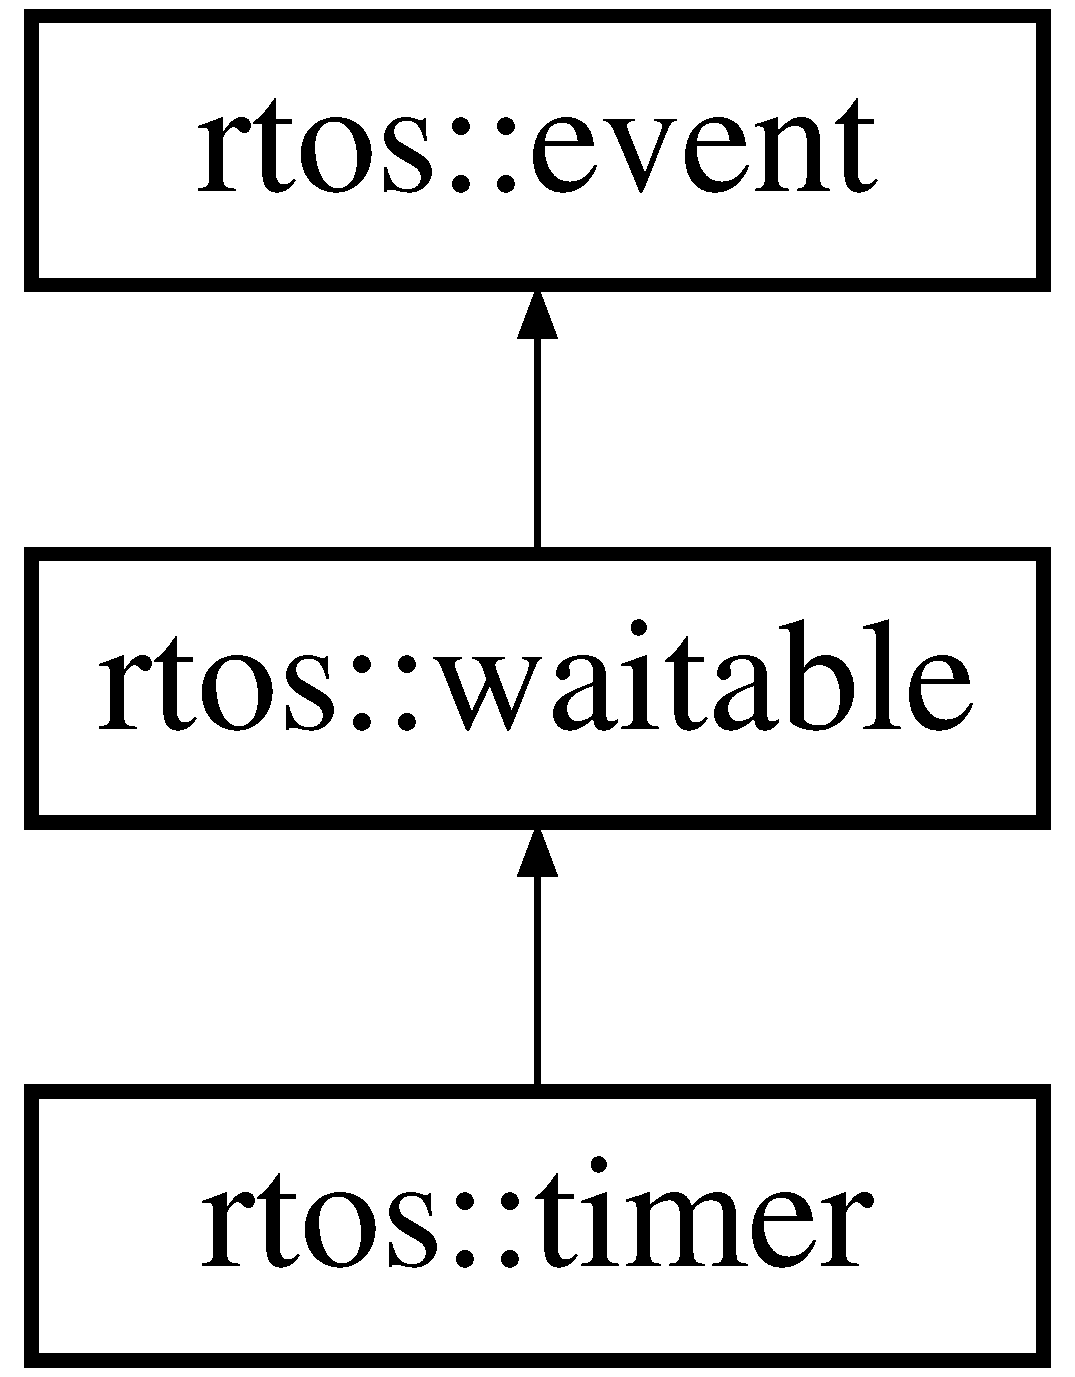
\includegraphics[height=3.000000cm]{classrtos_1_1timer}
\end{center}
\end{figure}
\subsection*{Public Member Functions}
\begin{DoxyCompactItemize}
\item 
\hyperlink{classrtos_1_1timer_a6c1cdeef312f1ed2b946097ef9196483}{timer} (\hyperlink{classrtos_1_1task__base}{task\+\_\+base} $\ast$\hyperlink{classrtos_1_1event_aa83745aabc941145f00386fd63f6b557}{t}, const char $\ast$name=\char`\"{}\char`\"{})\hypertarget{classrtos_1_1timer_a6c1cdeef312f1ed2b946097ef9196483}{}\label{classrtos_1_1timer_a6c1cdeef312f1ed2b946097ef9196483}

\begin{DoxyCompactList}\small\item\em create a timer for task t, specify its name \end{DoxyCompactList}\item 
void \hyperlink{classrtos_1_1timer_a8b5641b2d3cc0a5c9b48de1e5f7d0930}{set} (unsigned long int time)
\item 
void \hyperlink{classrtos_1_1timer_ac67cee76f7fdff1e95341a805d2d9748}{cancel} (void)
\begin{DoxyCompactList}\small\item\em stop and clear the timer \end{DoxyCompactList}\item 
void \hyperlink{classrtos_1_1timer_a4f80789abed43247008431021a2525b6}{print} (hwlib\+::ostream \&s, bool header=true) const \hypertarget{classrtos_1_1timer_a4f80789abed43247008431021a2525b6}{}\label{classrtos_1_1timer_a4f80789abed43247008431021a2525b6}

\begin{DoxyCompactList}\small\item\em print the timer (for debugging) \end{DoxyCompactList}\end{DoxyCompactItemize}
\subsection*{Friends}
\begin{DoxyCompactItemize}
\item 
class {\bfseries rtos}\hypertarget{classrtos_1_1timer_a2a7bcfc34141352757ad672e3ecd099f}{}\label{classrtos_1_1timer_a2a7bcfc34141352757ad672e3ecd099f}

\end{DoxyCompactItemize}
\subsection*{Additional Inherited Members}


\subsection{Detailed Description}
one-\/short timer 

A (one-\/shot) timer is a special type of flag, which can be instructed to set itself after a fixed amount of time. The amount of time is supplied with the \hyperlink{classrtos_1_1waitable_a3f1c5cfb702d4bd50b91fab1ab355bc0}{timer\+::set()} call. This call starts the timer. A timer that is running (waiting for its timeout to expire) can be canceled by the \hyperlink{classrtos_1_1timer_ac67cee76f7fdff1e95341a805d2d9748}{timer\+::cancel()} call. When a timer that is already running is set again the previous timeout is overwritten by the new one. The suspend/resume state of its owner taks has no effect on a timer\+: even when the task is suspended the timer will run to its timeout and set isetlf. But of course the task, being suspended, will not be able to react. 

\subsection{Member Function Documentation}
\index{rtos\+::timer@{rtos\+::timer}!cancel@{cancel}}
\index{cancel@{cancel}!rtos\+::timer@{rtos\+::timer}}
\subsubsection[{\texorpdfstring{cancel(void)}{cancel(void)}}]{\setlength{\rightskip}{0pt plus 5cm}void rtos\+::timer\+::cancel (
\begin{DoxyParamCaption}
\item[{void}]{}
\end{DoxyParamCaption}
)}\hypertarget{classrtos_1_1timer_ac67cee76f7fdff1e95341a805d2d9748}{}\label{classrtos_1_1timer_ac67cee76f7fdff1e95341a805d2d9748}


stop and clear the timer 

Stop the timer (when it was running), and clears its (when it was set). \index{rtos\+::timer@{rtos\+::timer}!set@{set}}
\index{set@{set}!rtos\+::timer@{rtos\+::timer}}
\subsubsection[{\texorpdfstring{set(unsigned long int time)}{set(unsigned long int time)}}]{\setlength{\rightskip}{0pt plus 5cm}void rtos\+::timer\+::set (
\begin{DoxyParamCaption}
\item[{unsigned long int}]{time}
\end{DoxyParamCaption}
)}\hypertarget{classrtos_1_1timer_a8b5641b2d3cc0a5c9b48de1e5f7d0930}{}\label{classrtos_1_1timer_a8b5641b2d3cc0a5c9b48de1e5f7d0930}
Start the timer\+: it will set itself after the indicated timeout, starting from now. When the timer was already running the previous timout is overwritten. 

The documentation for this class was generated from the following files\+:\begin{DoxyCompactItemize}
\item 
rtos.\+hpp\item 
rtos.\+cpp\end{DoxyCompactItemize}

\hypertarget{classrtos_1_1waitable}{}\section{rtos\+:\+:waitable Class Reference}
\label{classrtos_1_1waitable}\index{rtos\+::waitable@{rtos\+::waitable}}


abstract thing that a task can wait for  




{\ttfamily \#include $<$rtos.\+hpp$>$}

Inheritance diagram for rtos\+:\+:waitable\+:\begin{figure}[H]
\begin{center}
\leavevmode
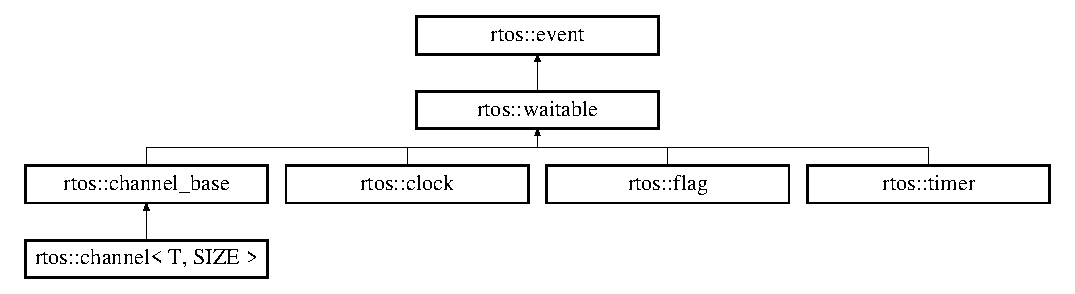
\includegraphics[height=3.500000cm]{classrtos_1_1waitable}
\end{center}
\end{figure}
\subsection*{Public Member Functions}
\begin{DoxyCompactItemize}
\item 
virtual void \hyperlink{classrtos_1_1waitable_ac4630398f50ba7e661a64bfc491ffa10}{clear} (void)
\begin{DoxyCompactList}\small\item\em clear the waitable \end{DoxyCompactList}\end{DoxyCompactItemize}
\subsection*{Protected Member Functions}
\begin{DoxyCompactItemize}
\item 
\hyperlink{classrtos_1_1waitable_aec600b639ba55717731d3c6cfe6ff8e6}{waitable} (\hyperlink{classrtos_1_1task__base}{task\+\_\+base} $\ast$\hyperlink{classrtos_1_1task}{task}, const char $\ast$name)
\begin{DoxyCompactList}\small\item\em constructor, specify owner and name \end{DoxyCompactList}\item 
void \hyperlink{classrtos_1_1waitable_a3f1c5cfb702d4bd50b91fab1ab355bc0}{set} (void)\hypertarget{classrtos_1_1waitable_a3f1c5cfb702d4bd50b91fab1ab355bc0}{}\label{classrtos_1_1waitable_a3f1c5cfb702d4bd50b91fab1ab355bc0}

\begin{DoxyCompactList}\small\item\em set the waitable \end{DoxyCompactList}\end{DoxyCompactItemize}
\subsection*{Friends}
\begin{DoxyCompactItemize}
\item 
class {\bfseries waitable\+\_\+set}\hypertarget{classrtos_1_1waitable_a0ee29d8961a0b67cea2c3fa76da116da}{}\label{classrtos_1_1waitable_a0ee29d8961a0b67cea2c3fa76da116da}

\end{DoxyCompactItemize}
\subsection*{Additional Inherited Members}


\subsection{Detailed Description}
abstract thing that a task can wait for 

The operation \hyperlink{classrtos_1_1waitable_ac4630398f50ba7e661a64bfc491ffa10}{clear()} is provided (virtual, the default only clears the waitable) \hyperlink{classrtos_1_1waitable_a3f1c5cfb702d4bd50b91fab1ab355bc0}{set()} is provided but private (not all waitables can be set by the user).

Waitable is an abstract class (there are no objects that are just a waitable). \hyperlink{classrtos_1_1flag}{flag}, \hyperlink{classrtos_1_1timer}{timer}, \hyperlink{classrtos_1_1clock}{clock} and \hyperlink{classrtos_1_1channel}{channel} are concrete classes that inherit from waitable. A waitable is always created for a particular task. A maximum of 31 waitables can be created for each task. (Actually the maximum is 32, but one waitable created internally to implement the sleep() call.) A waitable can be in two states\+: set or cleared. A waitable is initially cleared.

A task can wait for one, a subset, or all waitables created for it. The default is to wait for all waitables created for the task, the other variants are specified by supplying to the task\+:wait() call either a single waitable, or the sum (operator+) of the waitables you want to wait for. When one of the waitables that is waited for becomes set the wait() call clears that waitable and returns an event that compares equal to the waitable. (Note that some waitables, for instance the channel, can immediately set itself again.) The calling task can compare that event to the waitables to see which event happened. When more than one of the waited-\/for waitables is set the wait() call makes an arbitrary choice from these waitables. 

\subsection{Constructor \& Destructor Documentation}
\index{rtos\+::waitable@{rtos\+::waitable}!waitable@{waitable}}
\index{waitable@{waitable}!rtos\+::waitable@{rtos\+::waitable}}
\subsubsection[{\texorpdfstring{waitable(task\+\_\+base $\ast$task, const char $\ast$name)}{waitable(task_base *task, const char *name)}}]{\setlength{\rightskip}{0pt plus 5cm}rtos\+::waitable\+::waitable (
\begin{DoxyParamCaption}
\item[{{\bf task\+\_\+base} $\ast$}]{task, }
\item[{const char $\ast$}]{name}
\end{DoxyParamCaption}
)\hspace{0.3cm}{\ttfamily [protected]}}\hypertarget{classrtos_1_1waitable_aec600b639ba55717731d3c6cfe6ff8e6}{}\label{classrtos_1_1waitable_aec600b639ba55717731d3c6cfe6ff8e6}


constructor, specify owner and name 

The name is used for debugging only. 

\subsection{Member Function Documentation}
\index{rtos\+::waitable@{rtos\+::waitable}!clear@{clear}}
\index{clear@{clear}!rtos\+::waitable@{rtos\+::waitable}}
\subsubsection[{\texorpdfstring{clear(void)}{clear(void)}}]{\setlength{\rightskip}{0pt plus 5cm}virtual void rtos\+::waitable\+::clear (
\begin{DoxyParamCaption}
\item[{void}]{}
\end{DoxyParamCaption}
)\hspace{0.3cm}{\ttfamily [inline]}, {\ttfamily [virtual]}}\hypertarget{classrtos_1_1waitable_ac4630398f50ba7e661a64bfc491ffa10}{}\label{classrtos_1_1waitable_ac4630398f50ba7e661a64bfc491ffa10}


clear the waitable 

This is automatically doen when the waitable causes a \hyperlink{classrtos_1_1task__base_a2590ba76480cecaff66282516fbeb1bb}{task\+::wait()} call to return it. 

Reimplemented in \hyperlink{classrtos_1_1channel_a0a86102d13f98ef7258a3fadbc881abd}{rtos\+::channel$<$ T, S\+I\+Z\+E $>$}, and \hyperlink{classrtos_1_1clock_aa90115db325c074071ae956cb101f046}{rtos\+::clock}.



The documentation for this class was generated from the following files\+:\begin{DoxyCompactItemize}
\item 
rtos.\+hpp\item 
rtos.\+cpp\end{DoxyCompactItemize}

%--- End generated contents ---

% Index
\backmatter
\newpage
\phantomsection
\clearemptydoublepage
\addcontentsline{toc}{chapter}{Index}
\printindex

\end{document}
